\appendix
\clearpage{\renewcommand{\appendixname}{Anexos}

%===============================DOCENCIA==============================================

\chapter{Ejemplo de fichero para la importación de datos}
\begin{figure}[H]
	\centering
	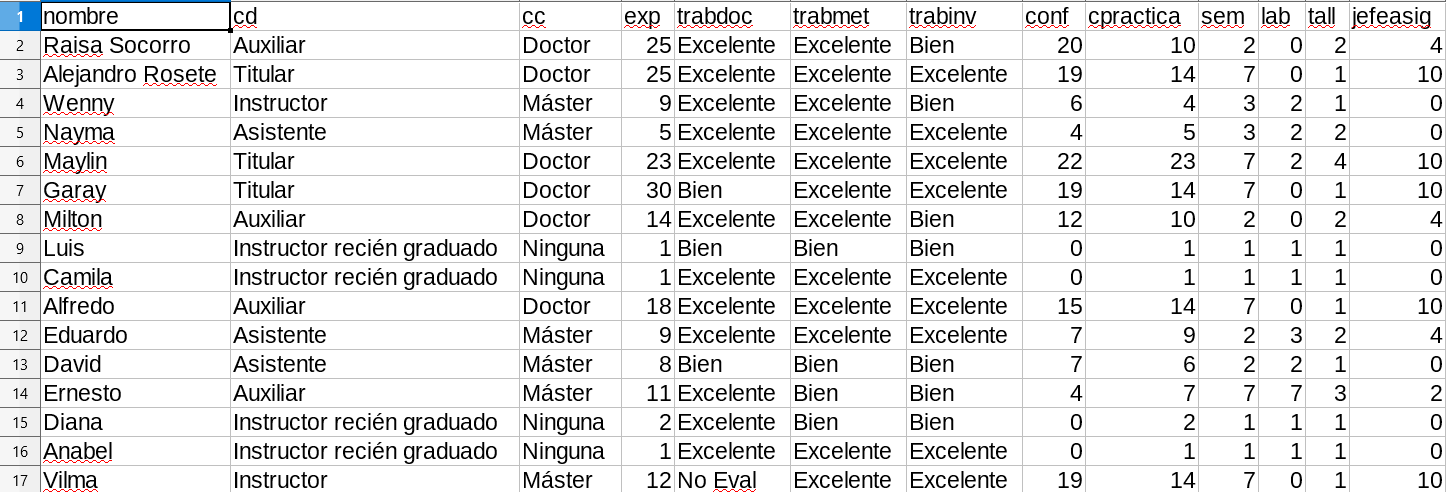
\includegraphics[width=.8\textwidth]{figuras/fichero-docencia.png}
	\caption{Fichero importar docencia} \label{fig:fichero-docencia}
\end{figure}

\begin{figure}[H]

	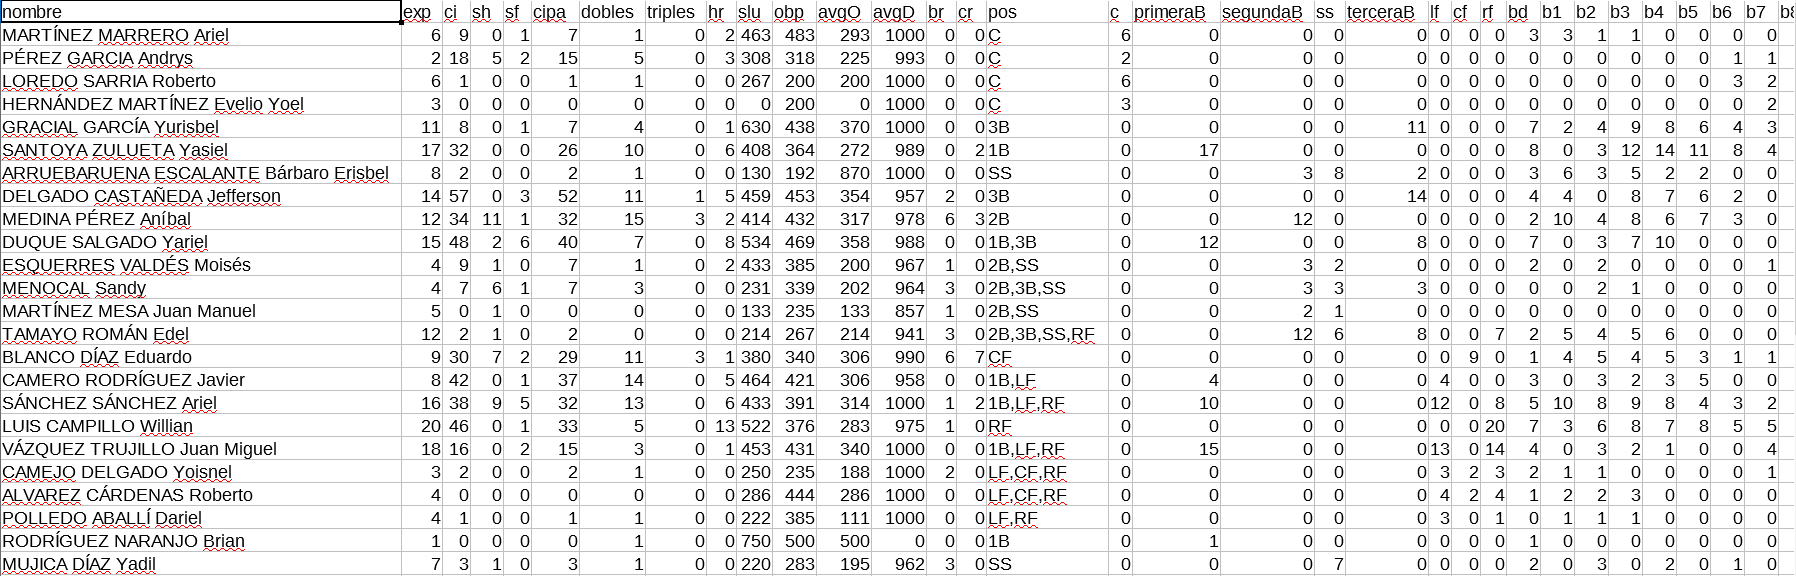
\includegraphics[width=\textwidth]{figuras/fichero-beisbol.png}
	\caption{Fichero importar béisbol} \label{fig:fichero-beisbol}
\end{figure}



\chapter{Pantalla de seleccionar el fichero y establecer grupo}
\begin{figure}[H]
	\centering
	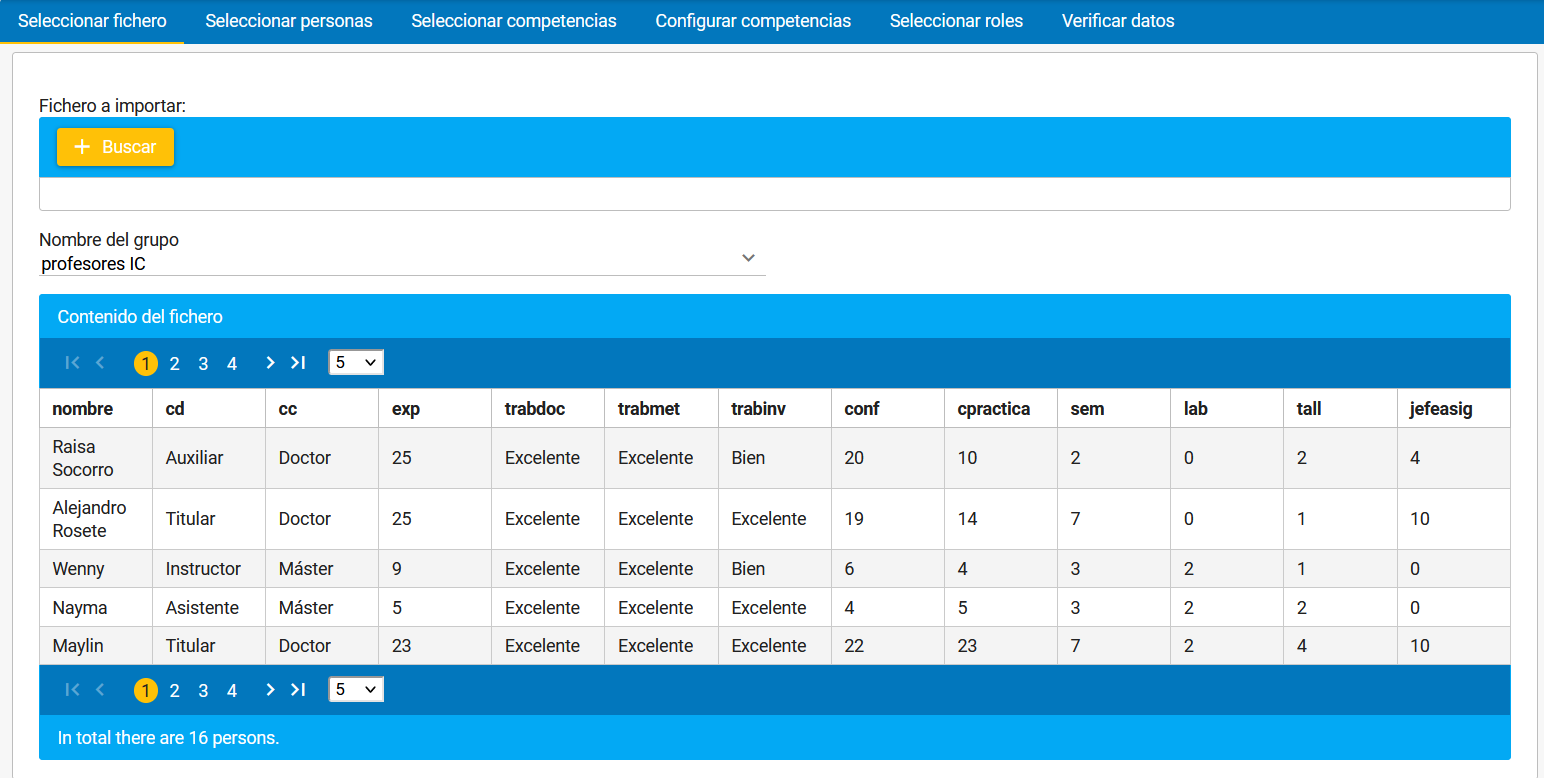
\includegraphics[width=\textwidth]{figuras/cargar_fichero_docencia.png}
	\caption{Pantalla cargar después de seleccionado el fichero y establecido el grupo (docencia)} \label{fig:cargar-fichero-docencia}
\end{figure}

\begin{figure}[H]
	\centering
	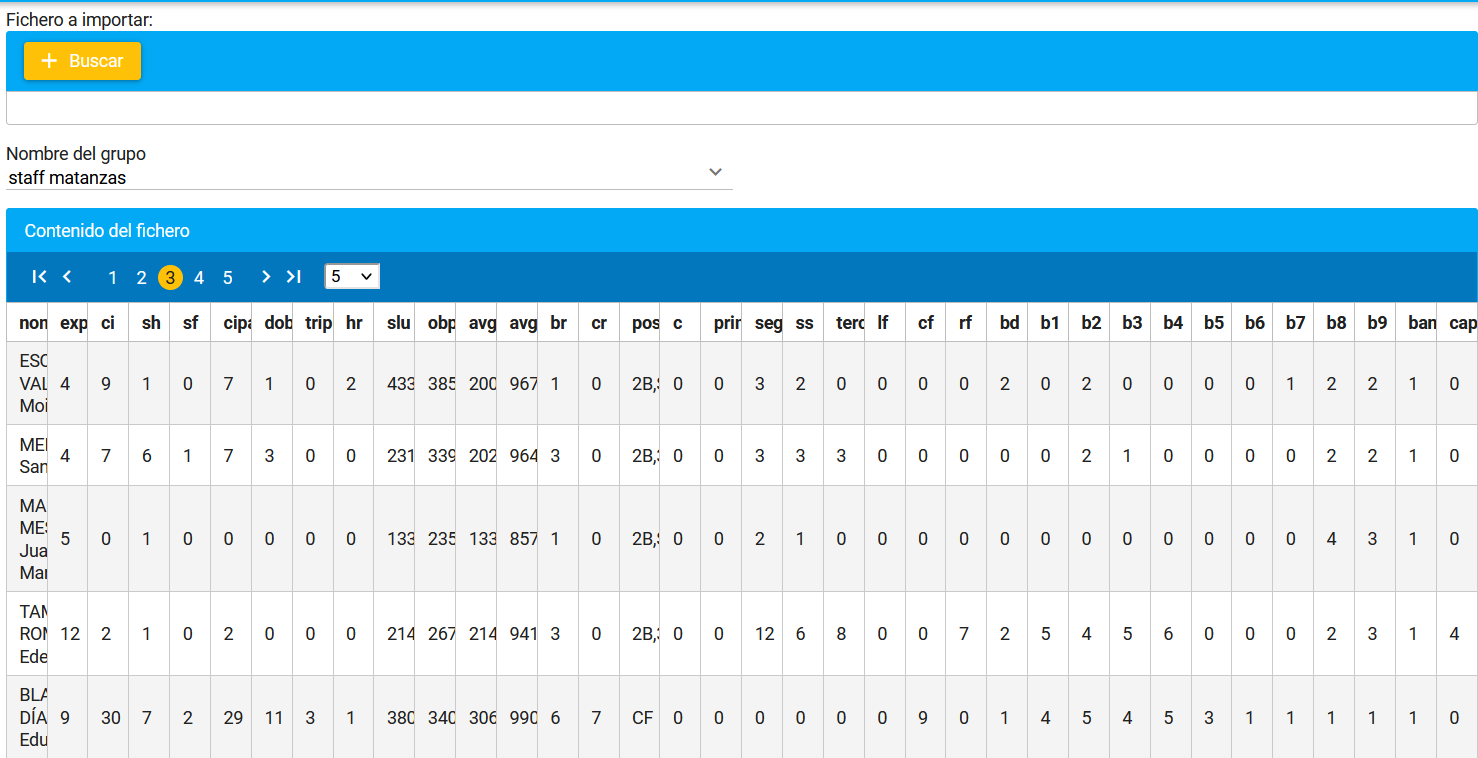
\includegraphics[width=\textwidth]{figuras/cargar_fichero_beisbol.png}
	\caption{Pantalla cargar después de seleccionado el fichero y establecido el grupo (béisbol)} \label{fig:cargar-fichero-beisbol}
\end{figure}


\chapter{Pantalla mapeo datos de las personas}
\begin{figure}[H]
	\centering
	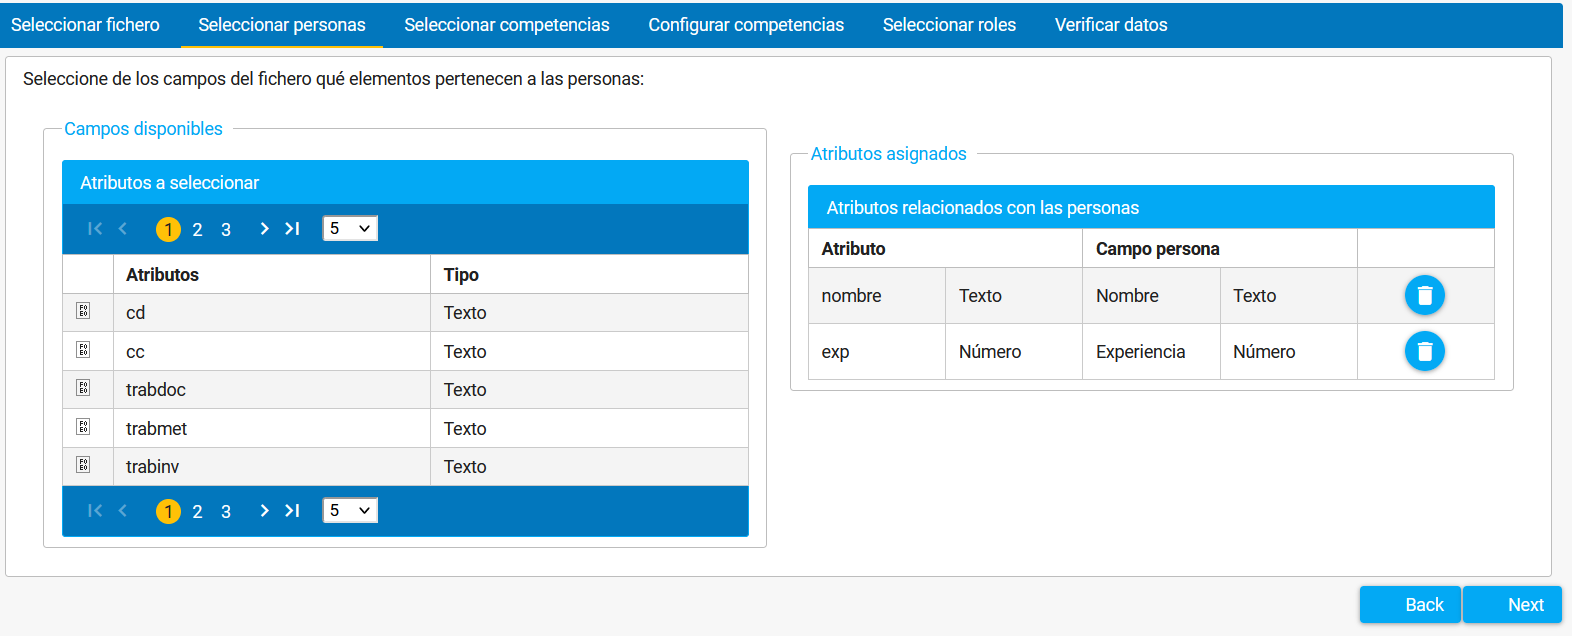
\includegraphics[width=\textwidth]{figuras/docencia_mapeo_atributos_personas.png}
	\caption{Asociar atributos del fichero a las personas (común para los dos problemas)} \label{fig:mapeo_atr_pers}
\end{figure}



%=======================Competencias=========================

%---------------------------DOCENCIA-----------------------------------------
\chapter{Pantalla configuración competencias}
\begin{figure}[H]
	\centering
	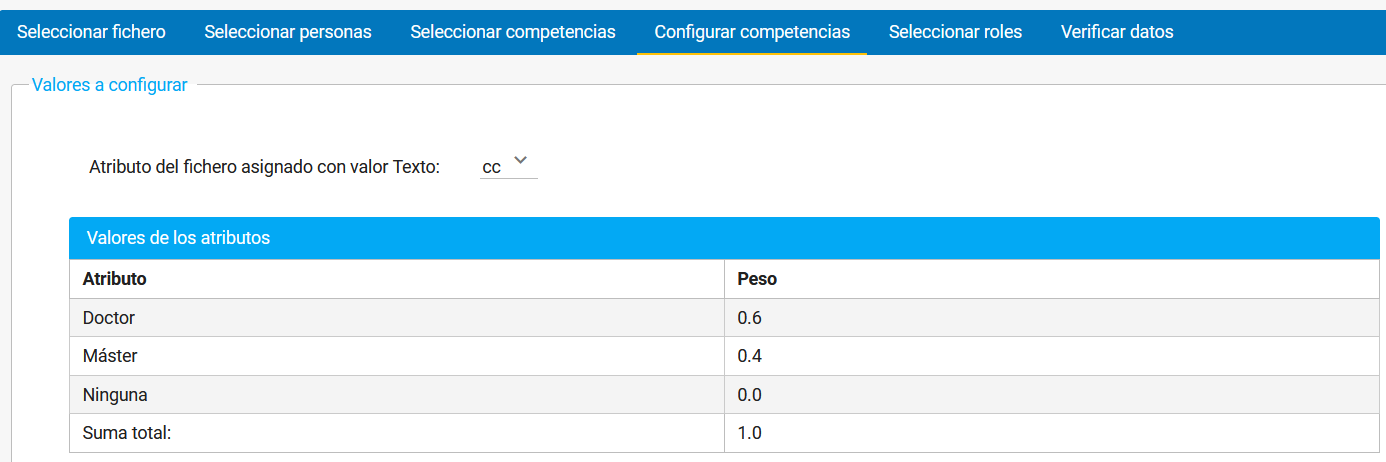
\includegraphics[width=\textwidth]{figuras/docencia_config_competencias_cc.png}
	\caption{Asociar peso a los valores del atributo cc (docencia)} \label{fig:conf_comp_cc_docencia}
\end{figure}

\begin{figure}[H]
	\centering
	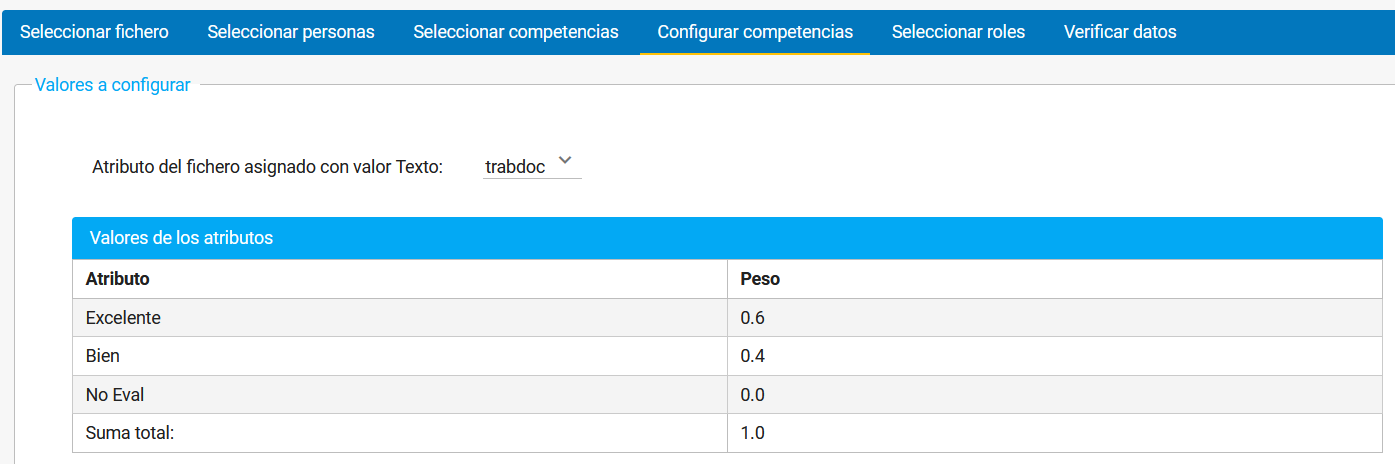
\includegraphics[width=\textwidth]{figuras/docencia_config_competencias_doc.png}
	\caption{Asociar peso a los valores del atributo trabdoc (docencia)} \label{fig:conf_comp_doc_docencia}
\end{figure}

\begin{figure}[H]
	\centering
	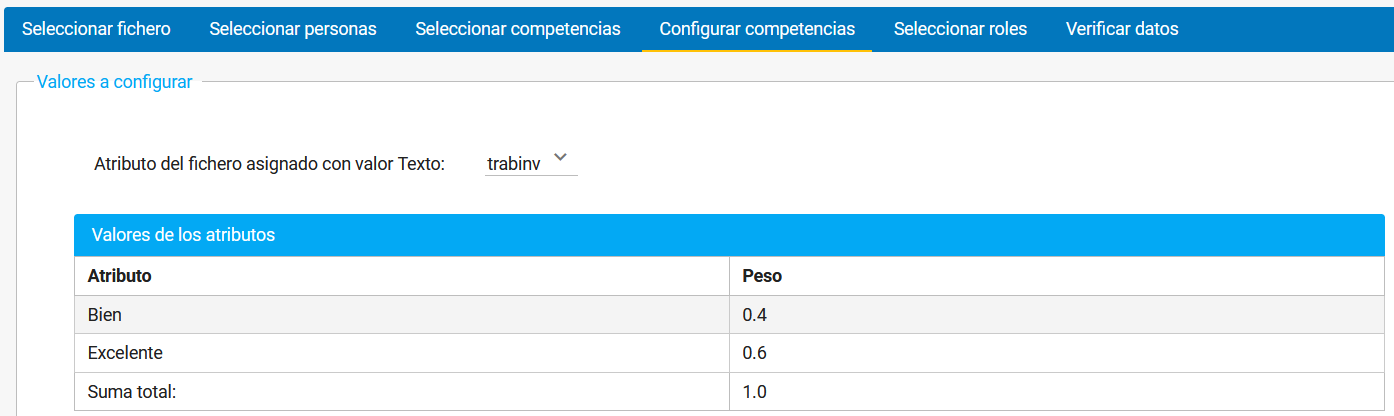
\includegraphics[width=\textwidth]{figuras/docencia_config_competencias_inv.png}
	\caption{Asociar peso a los valores del atributo trabinv (docencia)} \label{fig:conf_comp_inv_docencia}
\end{figure}

%----------------------------BEISBOL----------------------------------------

\begin{figure}[H]
	\centering
	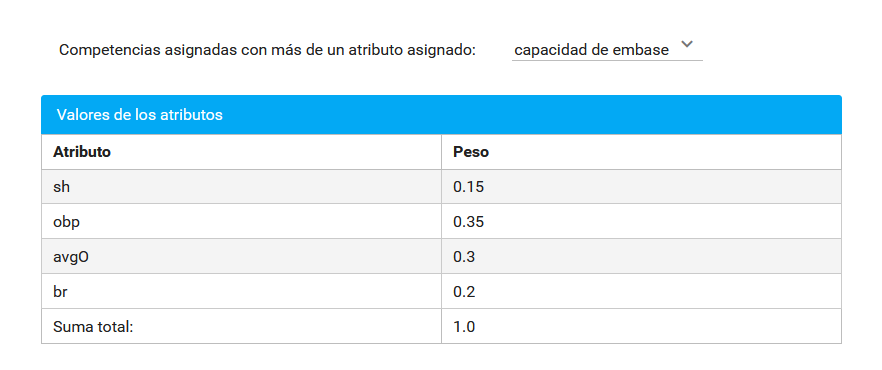
\includegraphics[width=\textwidth]{figuras/beisbol_conf_comp_ce.png}
	\caption{Asociar peso a los valores del atributo cc (béisbol)} \label{fig:conf_comp_ce_beisbol}
\end{figure}

\begin{figure}[H]
	\centering
	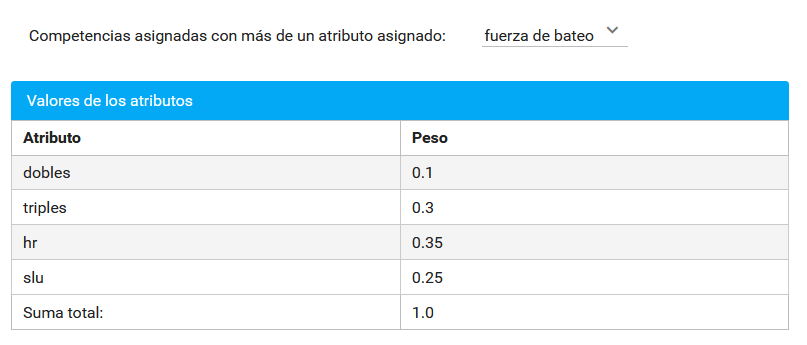
\includegraphics[width=\textwidth]{figuras/beisbol_conf_comp_fb.png}
	\caption{Asociar peso a los valores del atributo trabdoc (béisbol)} \label{fig:conf_comp_fb_beisbol}
\end{figure}

\begin{figure}[H]
	\centering
	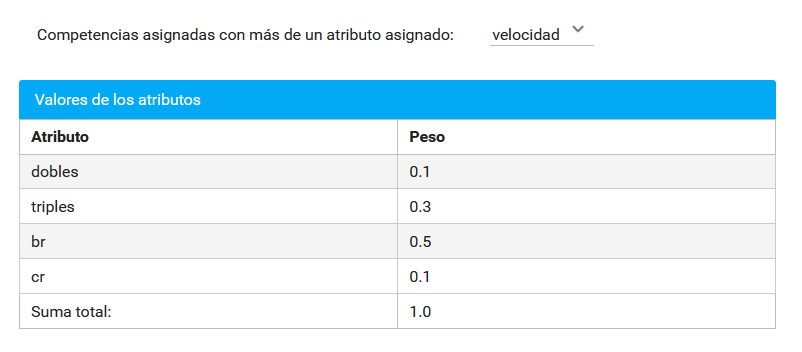
\includegraphics[width=\textwidth]{figuras/beisbol_conf_comp_v.png}
	\caption{Asociar peso a los valores del atributo trabinv (béisbol)} \label{fig:conf_comp_v_beisbol}
\end{figure}

%=======================Fin Competencias=========================

\chapter{Pantalla verificar datos}
\begin{figure}[H]
	\centering
	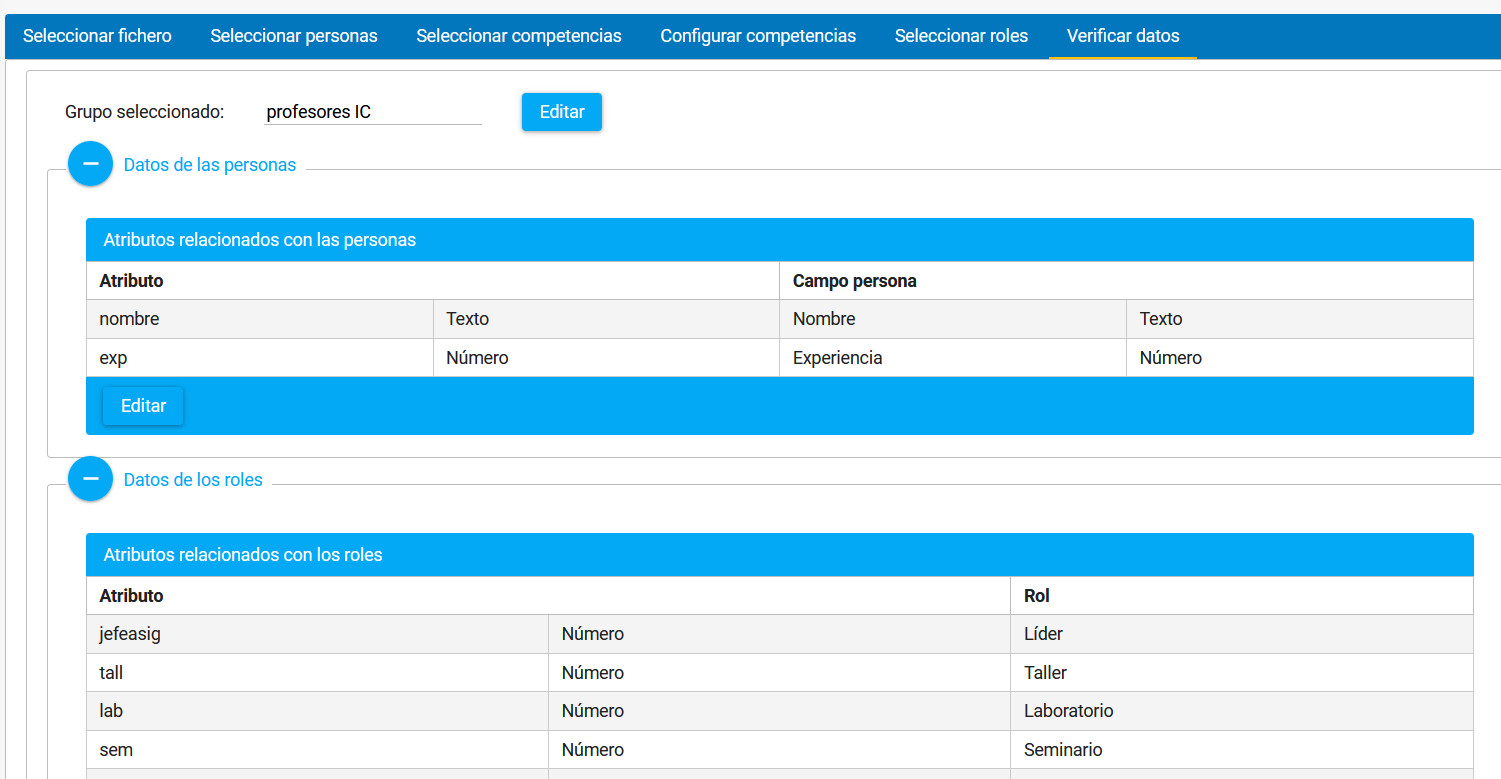
\includegraphics[width=\textwidth]{figuras/docencia_verificacion.png}
	\caption{Pantalla verificación de los datos (docencia)} \label{fig:verificar_datos_docencia}
\end{figure}

\begin{figure}[H]
	\centering
	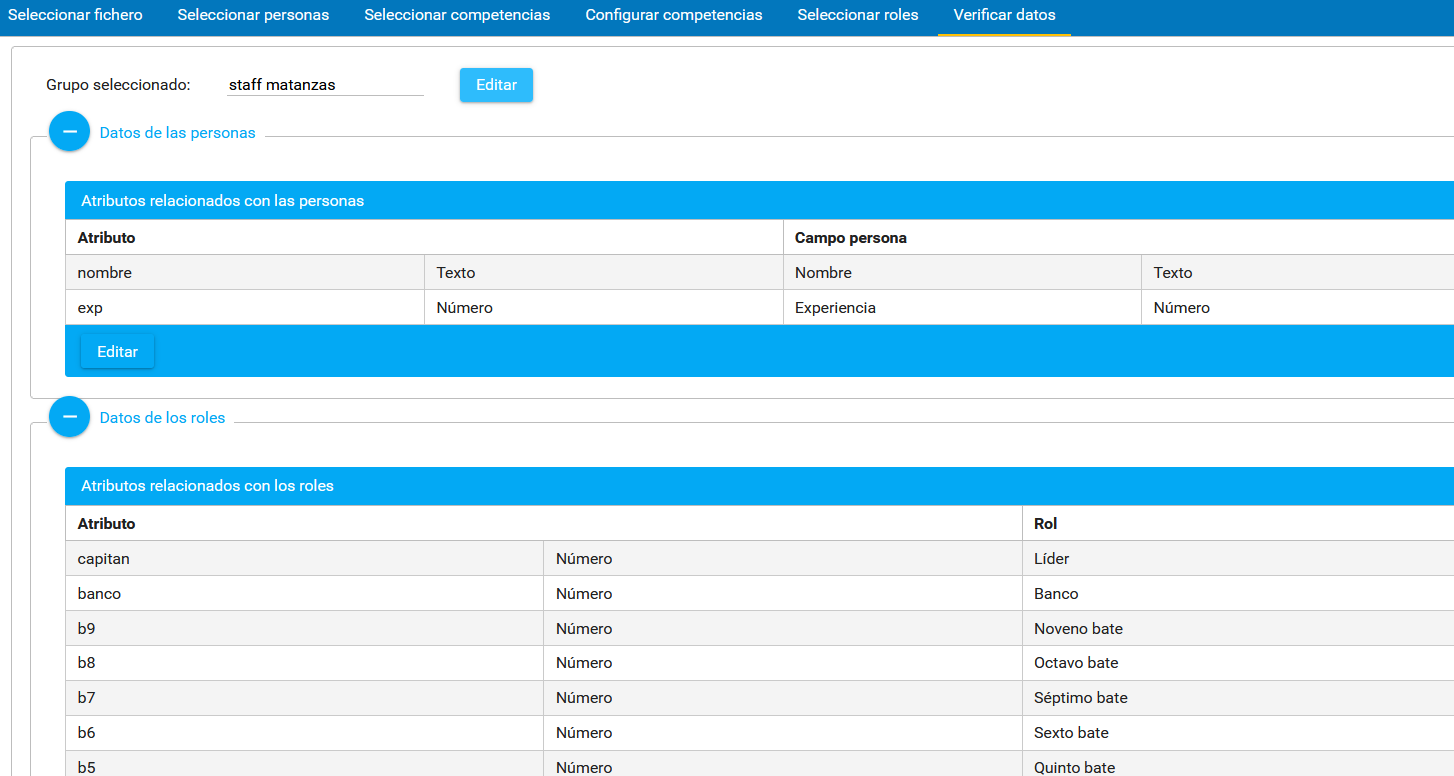
\includegraphics[width=\textwidth]{figuras/beisbol_verificacion.png}
	\caption{Pantalla verificación de los datos (béisbol)} \label{fig:verificar_datos_beisbol}
\end{figure}



\chapter{Pantalla mensaje información}
\begin{figure}[H]
	\centering
	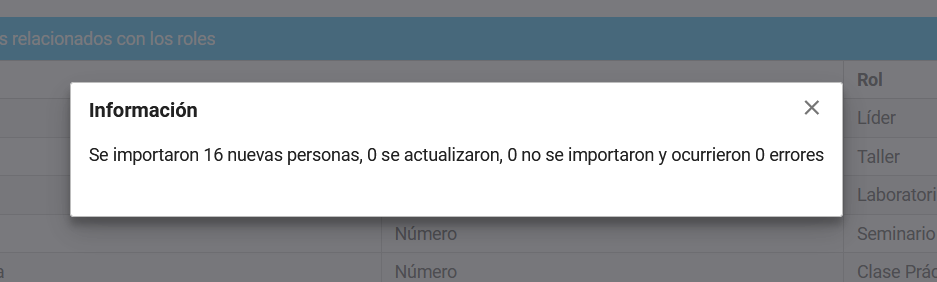
\includegraphics[width=\textwidth]{figuras/docencia_resultados.png}
	\caption{Mensaje de información después de importar (docencia)} \label{fig:resultados_docencia}
\end{figure}

\begin{figure}[H]
	\centering
	
\includegraphics[width=\textwidth]{figuras/beisbol_resultados.png}
	\caption{Mensaje de información después de importar (béisbol)} \label{fig:resultados_beisbol}
\end{figure}



\chapter{Pantalla lista de personas importadas}
\begin{figure}[H]
	\centering
	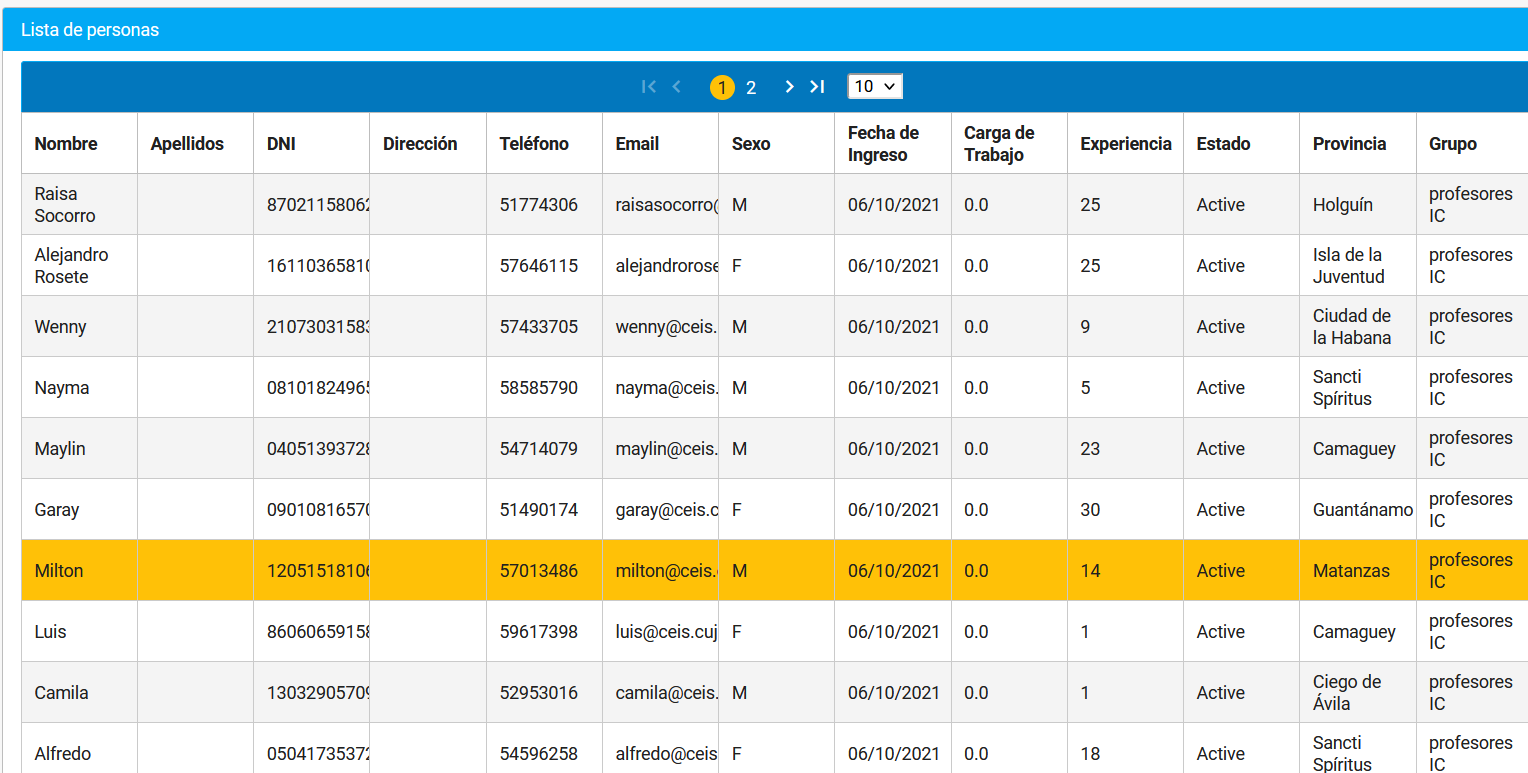
\includegraphics[width=\textwidth]{figuras/milton_seleccionado.png}
	\caption{Listado de personas importadas (docencia)} \label{fig:lista_profesores_docencia}
\end{figure}

\begin{figure}[H]
	\centering
	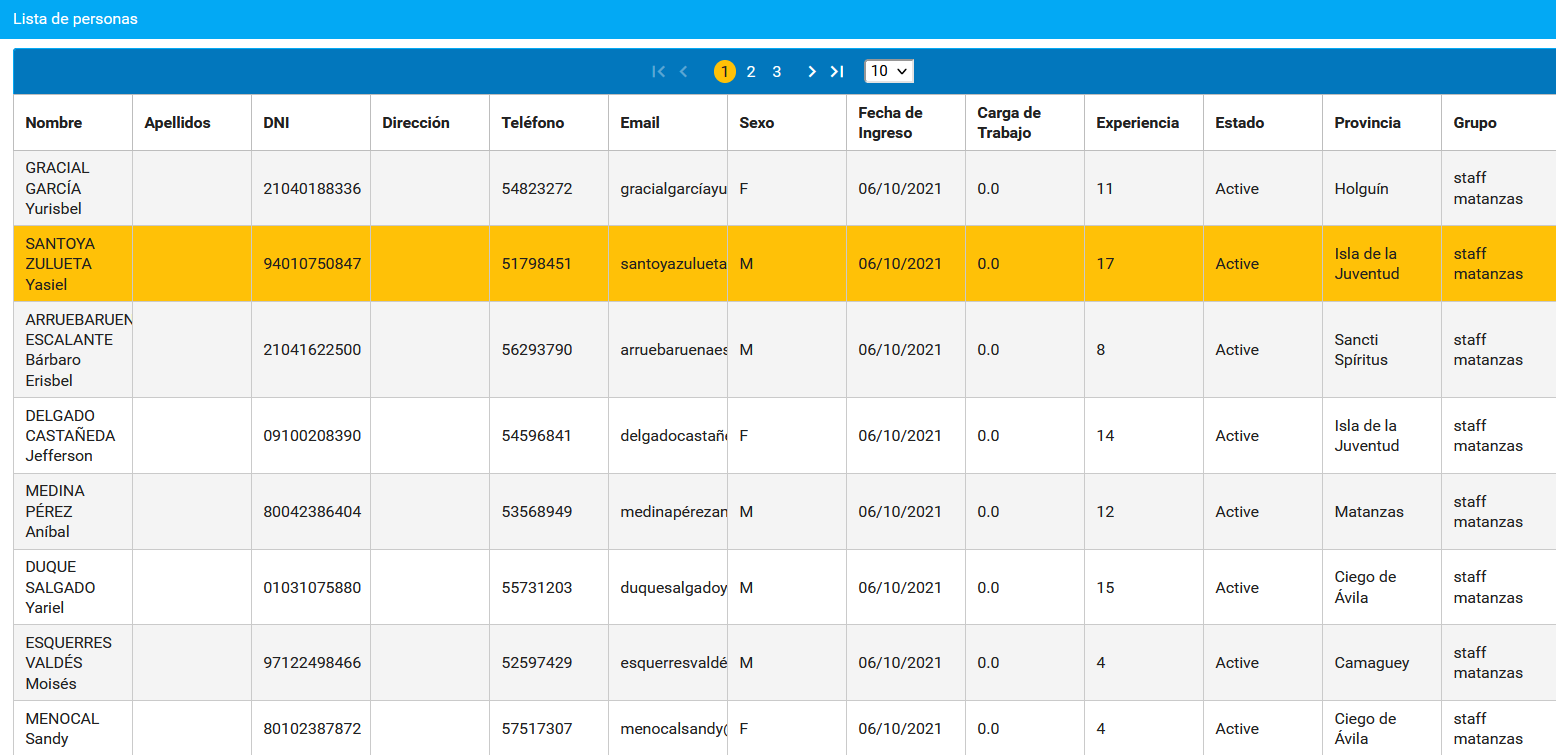
\includegraphics[width=\textwidth]{figuras/besibol_santoya_seleccionado.png}
	\caption{Listado de personas importadas (béisbol)} \label{fig:lista_jugadores_beisbol}
\end{figure}




\chapter{Pantalla competencias genéricas de una persona}
\begin{figure}[H]
	\centering
	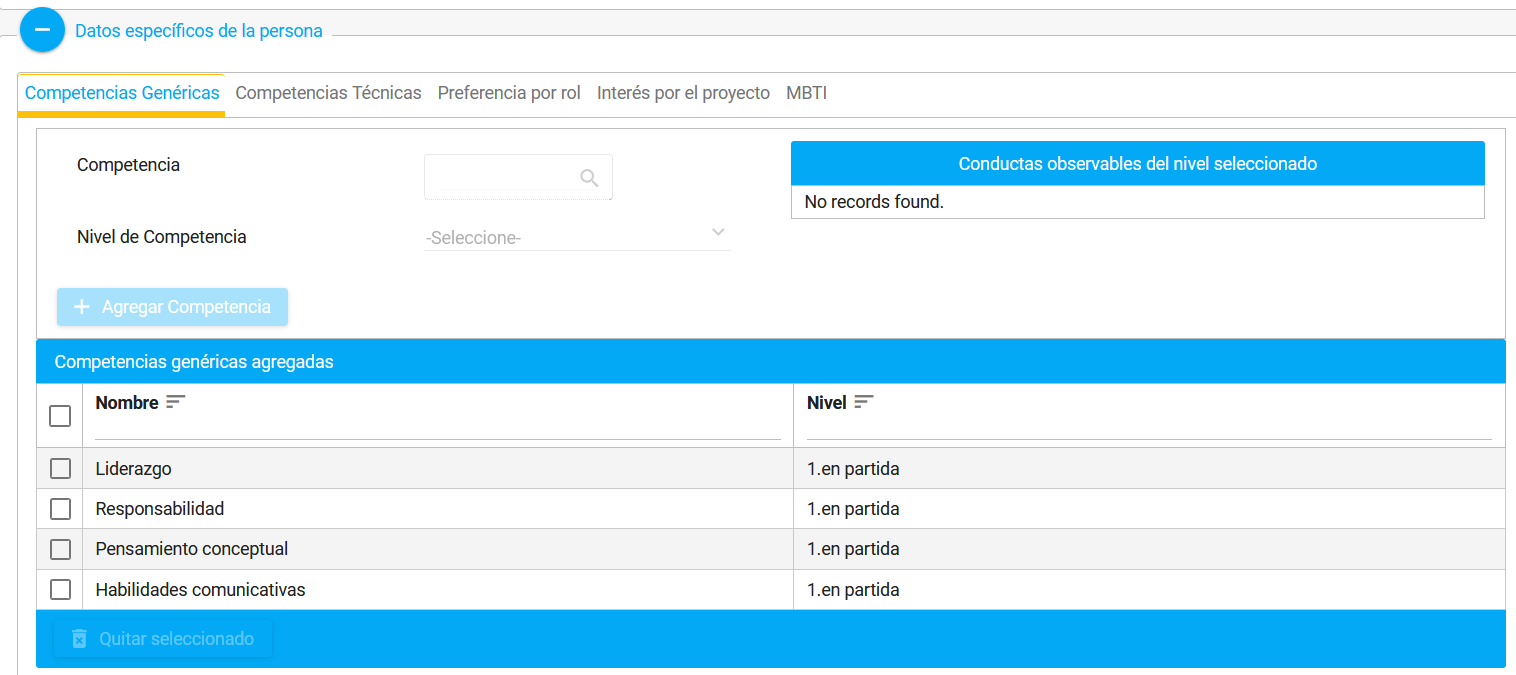
\includegraphics[width=\textwidth]{figuras/milton_comp_genericas.png}
	\caption{Competencias genéricas de Milton (docencia)} \label{fig:comp_genericas_docencia}
\end{figure}

\begin{figure}[H]
	\centering
	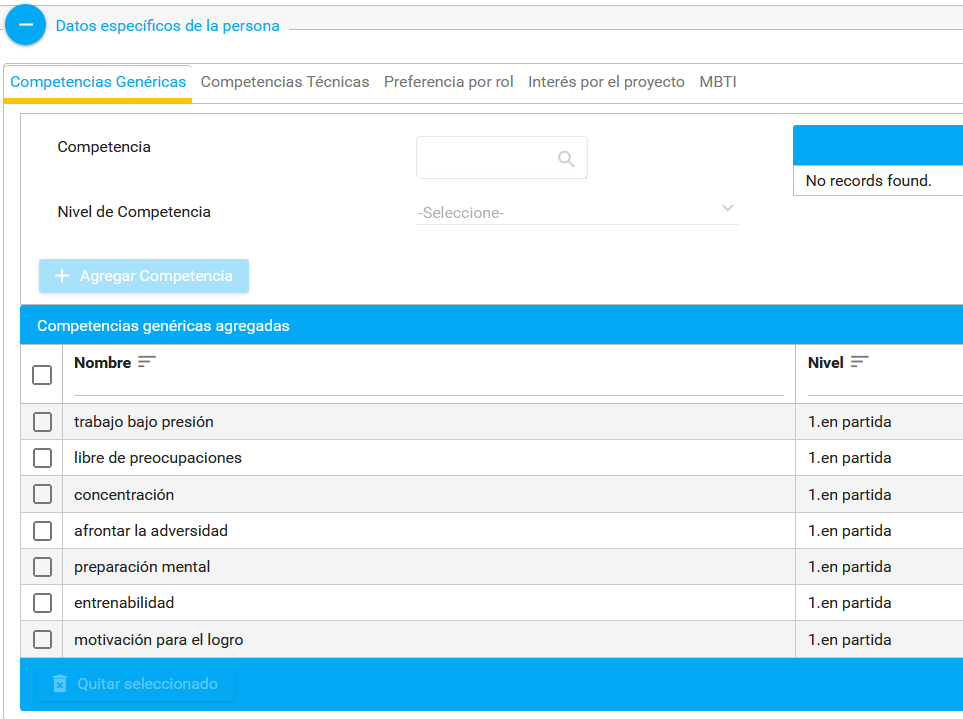
\includegraphics[width=\textwidth]{figuras/beisbol_santoya_compg.png}
	\caption{Competencias genéricas de Santoya (béisbol)} \label{fig:comp_genericas_beisbol}
\end{figure}


\chapter{Pantalla competencias técnicas de una persona}
\begin{figure}[H]
	\centering
	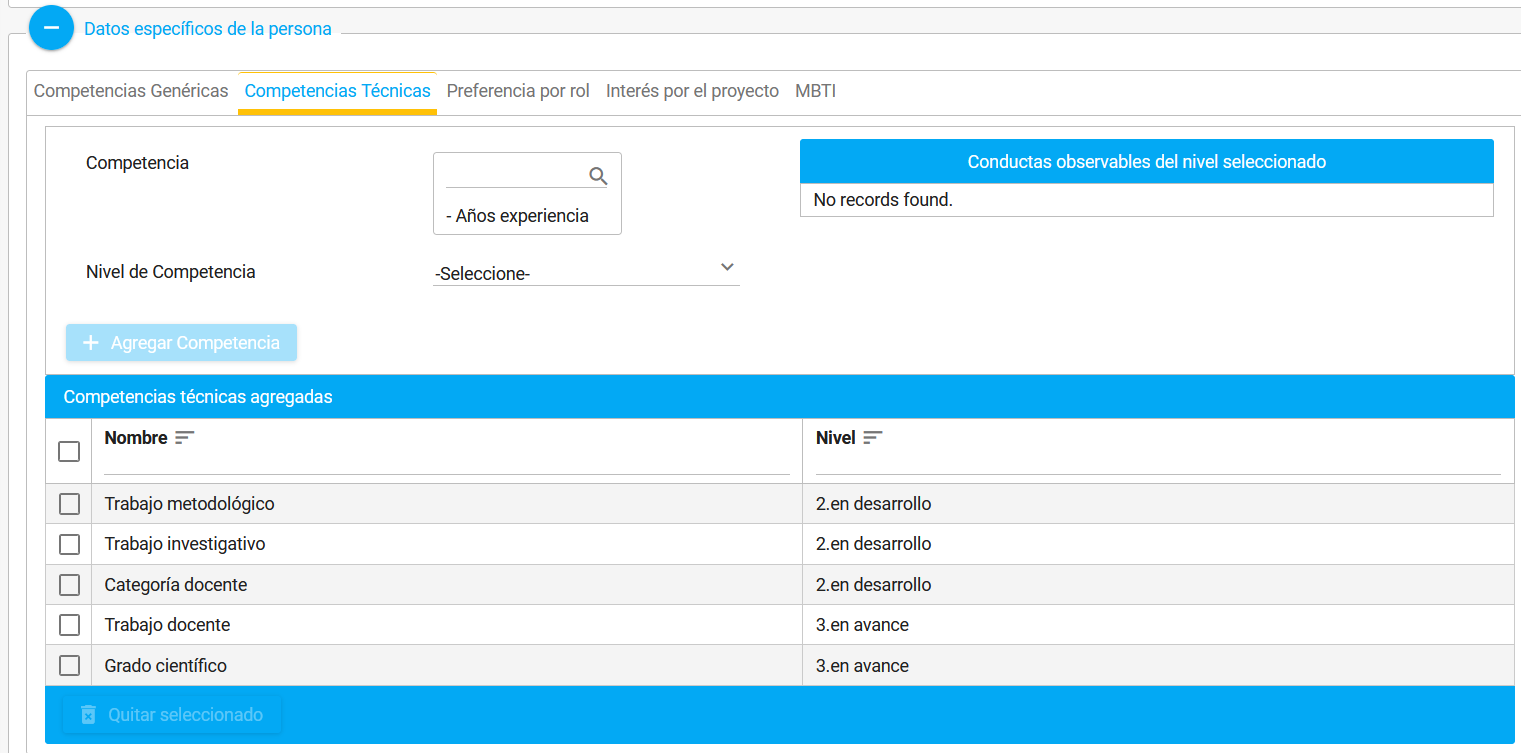
\includegraphics[width=\textwidth]{figuras/milton_competencias_tecnicas.png}
	\caption{Competencias técnicas de Milton (docencia)} \label{fig:comp_tecnicas_docencia}
\end{figure}

\begin{figure}[H]
	\centering
	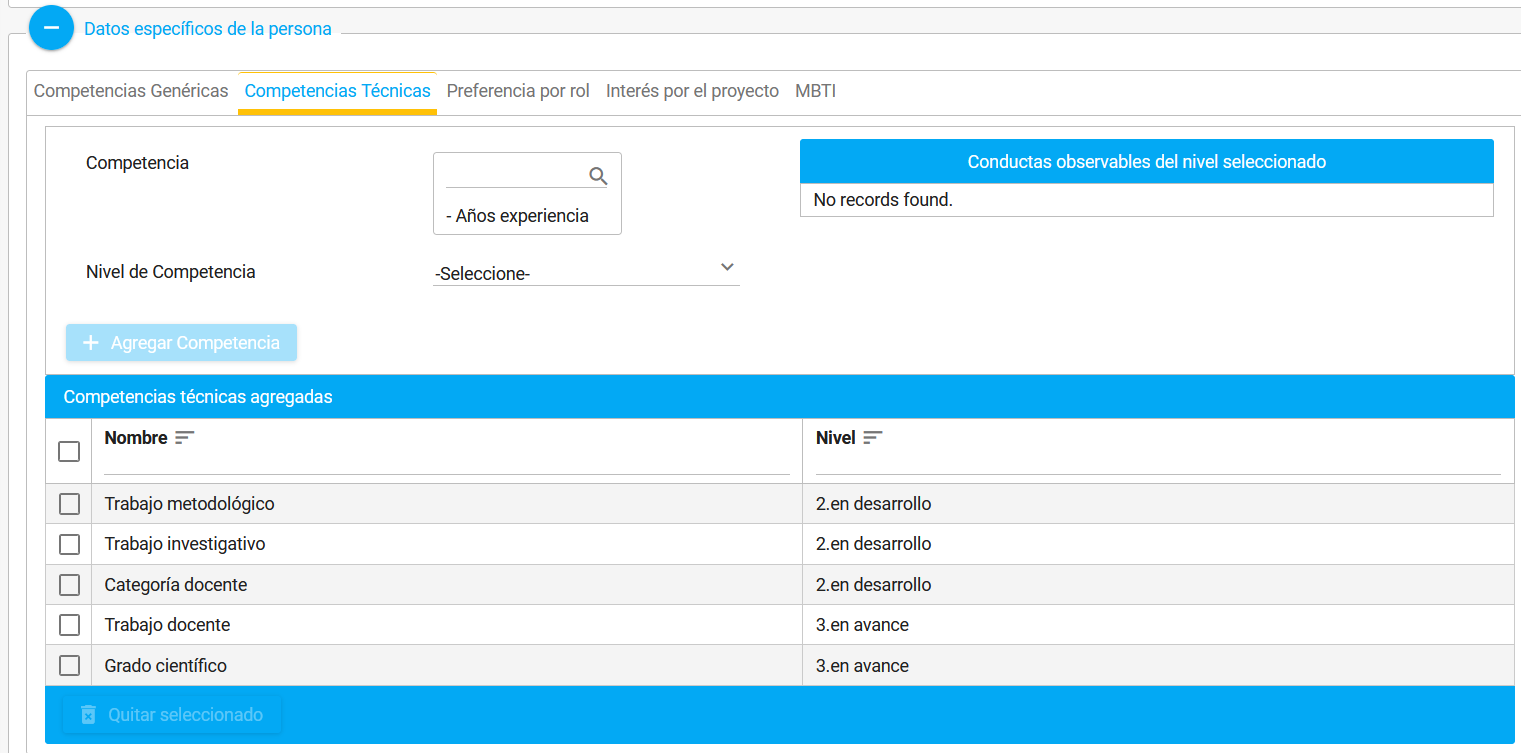
\includegraphics[width=\textwidth]{figuras/milton_competencias_tecnicas.png}
	\caption{Competencias técnicas de Santoya (béisbol)} \label{fig:comp_tecnicas_beisbol}
\end{figure}

\chapter{Pantalla preferencia por los roles de una persona}
\begin{figure}[H]
	\centering
	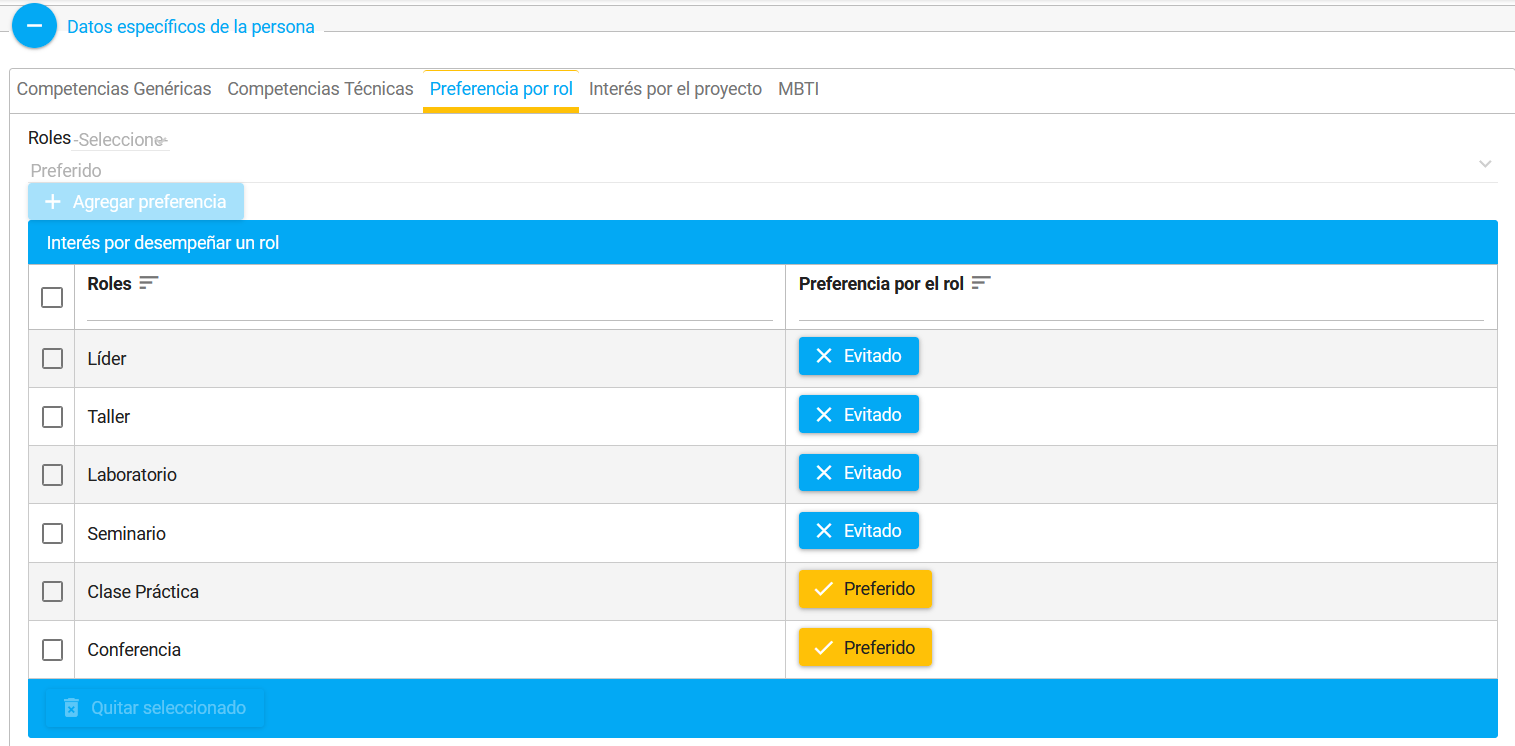
\includegraphics[width=\textwidth]{figuras/milton_preferencia_roles.png}
	\caption{Preferencia de Milton por los roles (docencia)} \label{fig:pref_roles_docencia}
\end{figure}

\begin{figure}[H]
	\centering
	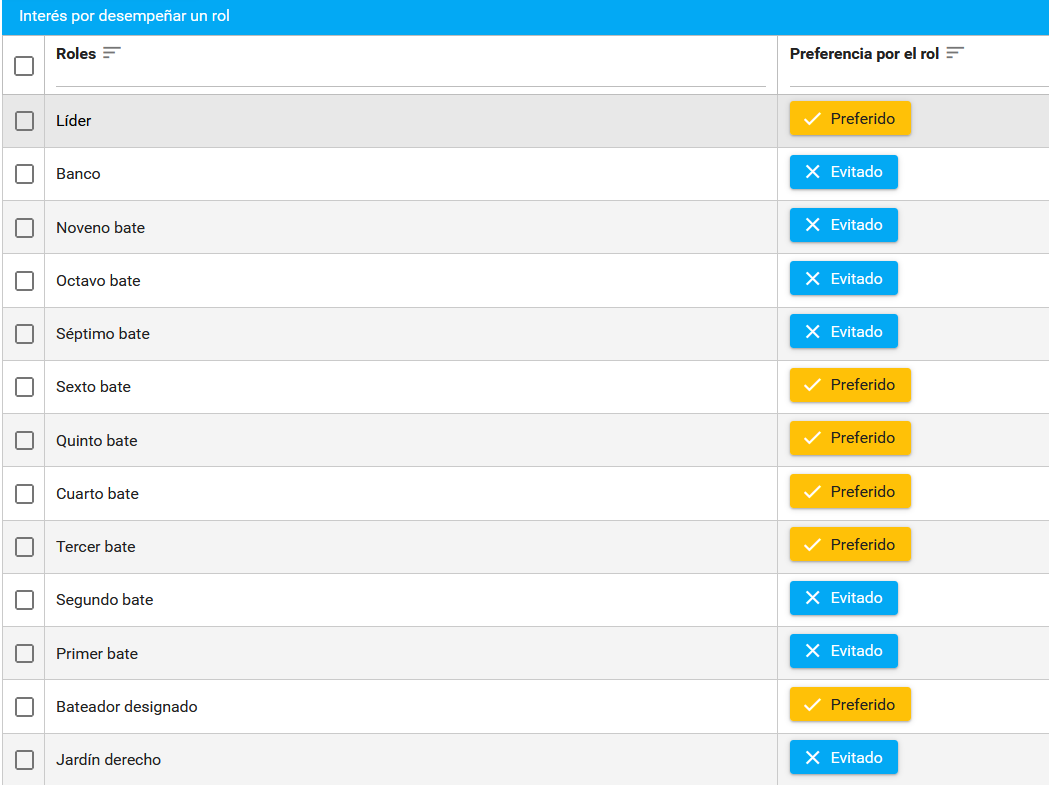
\includegraphics[width=\textwidth]{figuras/beisbol_santoya_roles.png}
	\caption{Preferencia de Santoya por los roles (béisbol)} \label{fig:pref_roles_beisbol}
\end{figure}

% configuración
\chapter{Pantalla de configuración de la importación}
\begin{figure}[H]
	\centering
	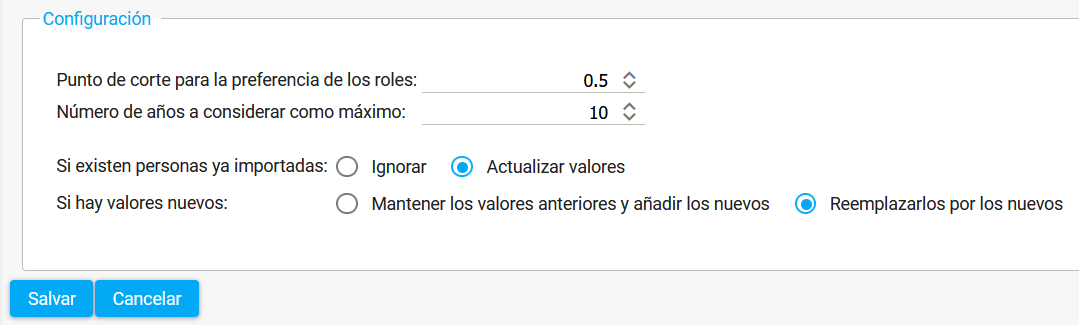
\includegraphics[width=\textwidth]{figuras/configuracion_importacion.png}
	\caption{Configuración de la importación} \label{fig:configuracion-problemas}
\end{figure}

\chapter{Configuración de las competencias requridas en los proyectos}

\begin{figure}[H]
	\centering
	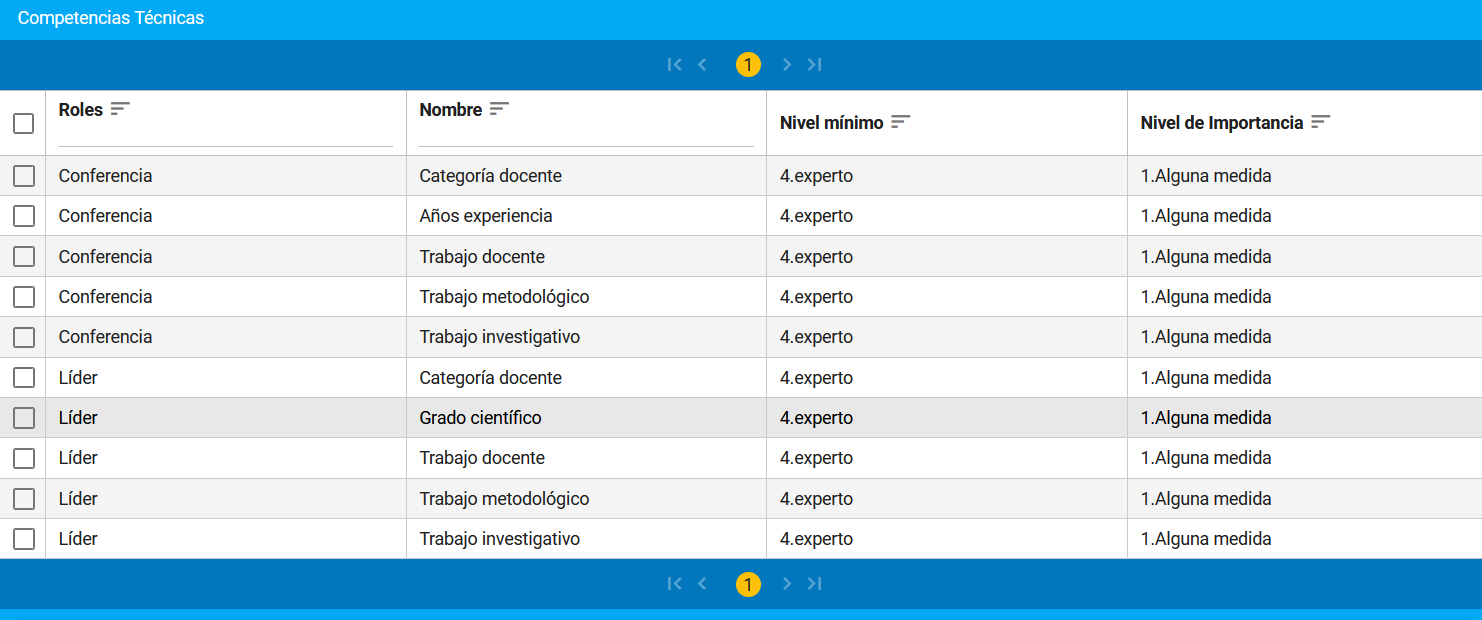
\includegraphics[width=\textwidth]{figuras/conf-roles-comp-asignatura.png}
	\caption{Configuración de las competenicas para todas las asignaturas} \label{fig:conf-roles-comp-asignatura}
\end{figure}

\begin{figure}[H]
	\centering
	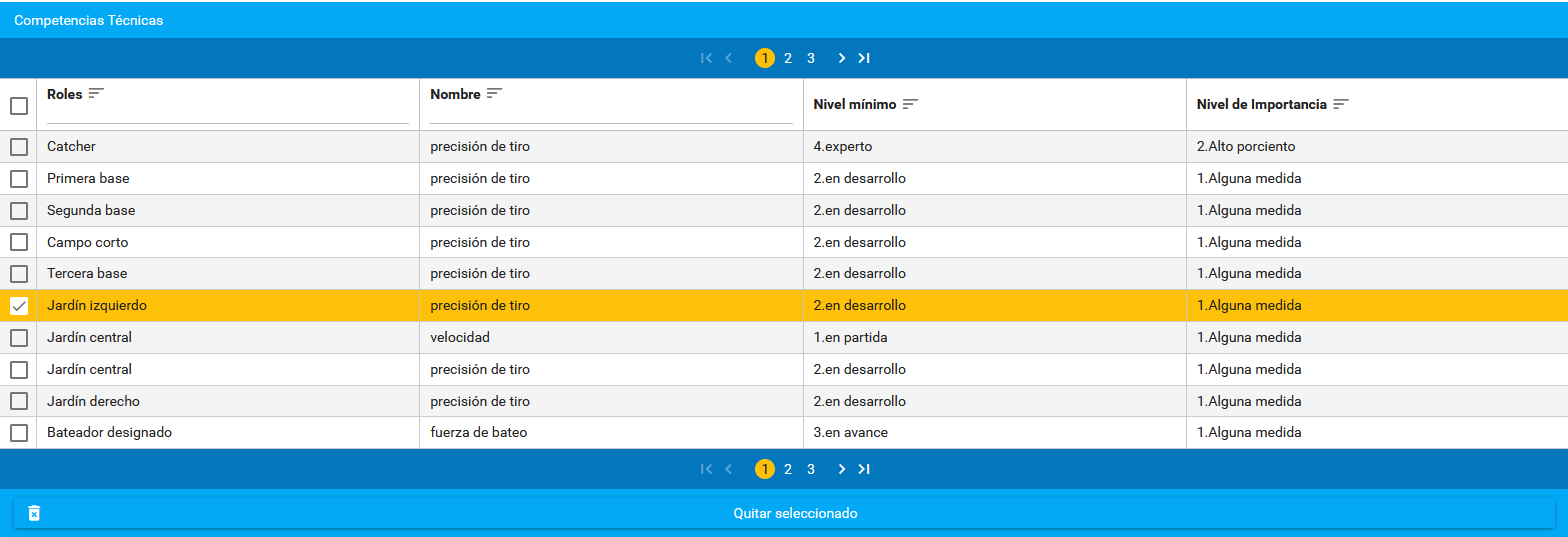
\includegraphics[width=\textwidth]{figuras/beisbol_conf_comp_rol1.png}
	\caption{Configuración de las competencias en los roles (béisbol)} \label{fig:conf-roles-comp-pelota}
\end{figure}

\begin{figure}[H]
	\centering
	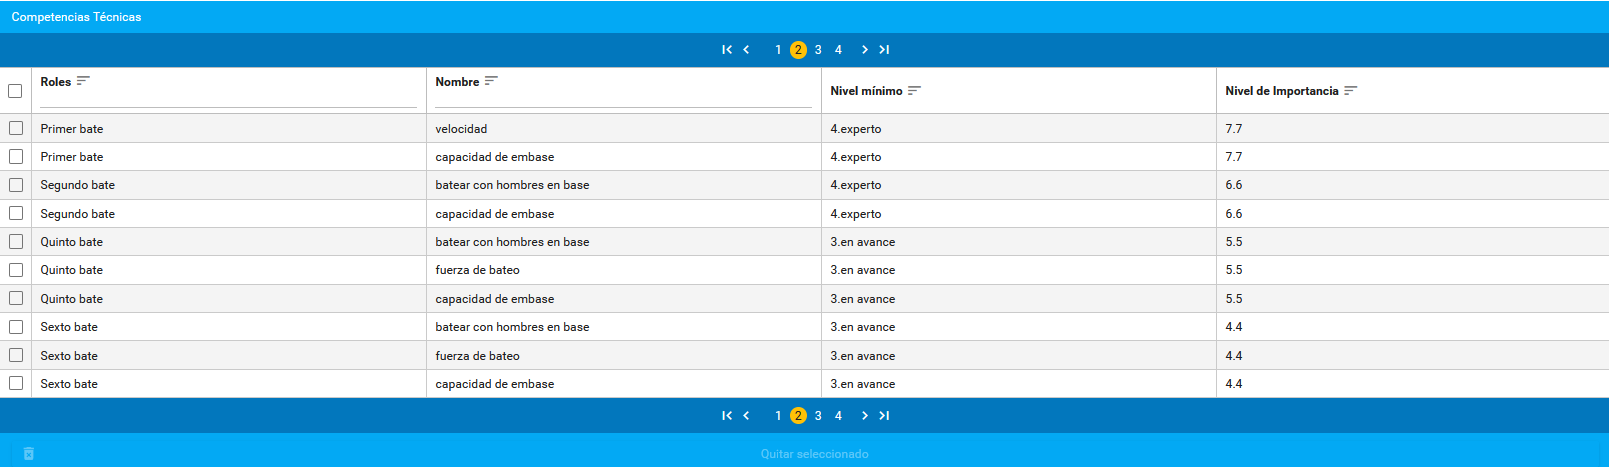
\includegraphics[width=\textwidth]{figuras/beisbol_conf_comp_rol2.png}
	\caption{Configuración de las competencias en los roles (béisbol)} \label{fig:conf-roles-comp-pelota1}
\end{figure}

\begin{figure}[H]
	\centering
	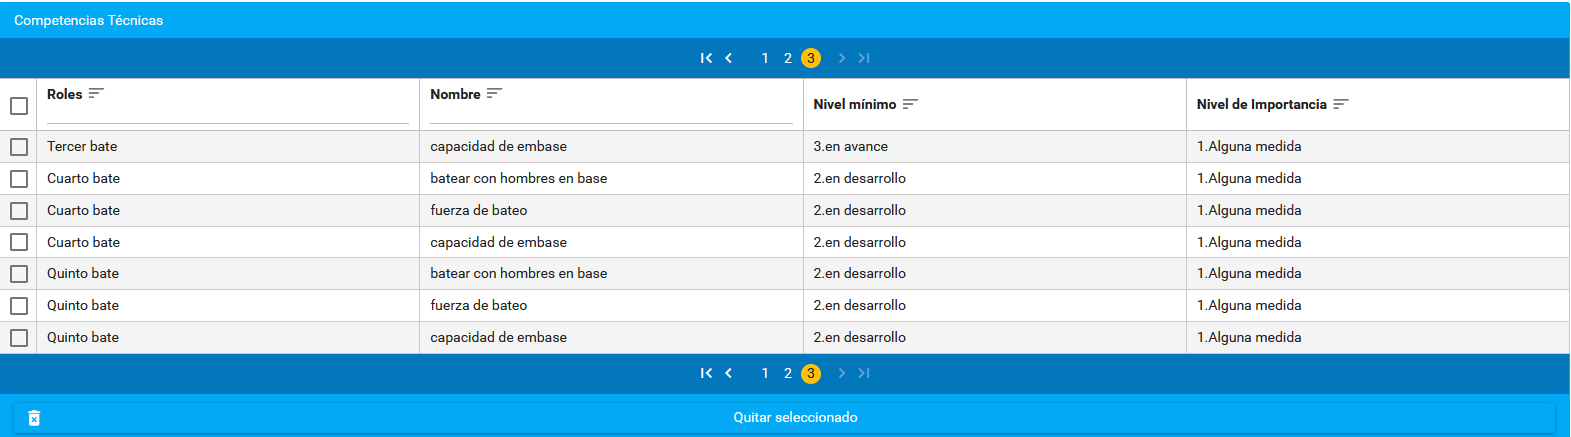
\includegraphics[width=\textwidth]{figuras/beisbol_conf_comp_rol3.png}
	\caption{Configuración de las competencias en los roles (béisbol)} \label{fig:conf-roles-comp-pelota2}
\end{figure}


\chapter{Nivel de las personas en las competencias}

\begin{table}[H]
	\centering
	\hspace{2cm}
	\caption{Nivel de los profesores por competencias: Trabajo docente (TD), Trabajo metodológico (TM), Trabajo investigativo (TI), Categoría docente (CD) y Grado científico (GC)}\label{table:nivel-pers-comp2}
	%	\scalebox{.87}{
	\begin{tabular}{l l l l l l}
		\toprule
		\multirow{2}{2cm}{\textbf{Profesor}} &           \multicolumn{4}{c}{\textbf{Competencias}}           &  \\ \cline{2-6}
		                                       & \textbf{TD}   & \textbf{TM}   & \textbf{TI}   & \textbf{CD}   & \textbf{GC}   \\ \midrule
		Wenny                                  & Experto       & Experto       & En desarrollo & En desarrollo & En avance     \\ \hline
		Nayma                                  & Experto       & Experto       & Experto       & En avance     & En avance     \\ \hline
		Garay                                  & En avance     & Experto       & Experto       & Experto       & Experto       \\ \hline
		Milton                                 & Experto       & Experto       & En desarrollo & Experto       & Experto       \\ \hline
		Alfredo                                & Experto       & Experto       & Experto       & Experto       & Experto       \\ \hline
		Eduardo                                & Experto       & Experto       & Experto       & En avance     & En avance     \\ \hline
		David                                  & En avance     & En desarrollo & En desarrollo & En avance     & En avance     \\ \hline
		Ernesto                                & Experto       & En desarrollo & En desarrollo & Experto       & En avance     \\ \hline
		Diana                                  & Experto       & En desarrollo & En desarrollo & En partida    & En desarrollo \\ \hline
		Anabel                                 & Experto       & Experto       & Experto       & En partida    & En desarrollo \\ \hline
		Vilma                                  & En desarrollo & Experto       & Experto       & En desarrollo & En avance     \\ \bottomrule
	\end{tabular}
	%}
\end{table}

\begin{table}[H]
	\centering
	%	\hspace{-4cm}
	\caption{Nivel de los jugadores en las competencias: Batear con hombres en base (B), Fuerza de bateo (F), Precisión de tiro (P), Capacidad de embase (E) y Velocidad (V)}\label{table:nivel-jugadores-comp2}
	\scalebox{.6}{
		\begin{tabular}{ p{2.6cm} c c c c c }
			\toprule
			\multirow{2}{2.5cm}{\textbf{Jugador}} &                 \multicolumn{5}{c}{\textbf{Competencias}}                  \\ \cline{2-6}
			                                      & \textbf{B}    & \textbf{P} & \textbf{F}    & \textbf{V}    & \textbf{E}    \\ \midrule
			Ariel Martínez                        & En partida    & Experto    & En partida    & En partida    & En desarrollo \\ \hline
			Roberto Loredo                        & En partida    & Experto    & En partida    & En partida    & En partida    \\ \hline
			Aníbal Medina                         & En avance     & Experto    & En avance     & Experto       & Experto       \\ \hline
			Evelio Hernández                      & En partida    & Experto    & En partida    & En partida    & En partida    \\ \hline
			Moisés Esquerres                      & En partida    & Experto    & En partida    & En partida    & En desarrollo \\ \hline
			Sandy Menocal                         & En partida    & Experto    & En partida    & En desarrollo & En desarrollo \\ \hline
			Juan Manuel Mesa                      & En partida    & Experto    & En partida    & En partida    & En desarrollo \\ \hline
			Edel Tamayo                           & En partida    & Experto    & En partida    & En partida    & En desarrollo \\ \hline
			Willian Luis                          & En desarrollo & Experto    & En avance     & En partida    & En desarrollo \\ \hline
			Juan Miguel                           & En desarrollo & Experto    & En partida    & En partida    & En desarrollo \\ \hline
			Yoisnel Camejo                        & En partida    & Experto    & En partida    & En partida    & En desarrollo \\ \hline
			Roberto Álvarez                       & En partida    & Experto    & En partida    & En partida    & En desarrollo \\ \hline
			Dariel Polledo                        & En partida    & Experto    & En partida    & En partida    & En desarrollo \\ \hline
			Brian Rodríguez                       & En partida    & En partida & En desarrollo & En partida    & En avance     \\ \hline
			Yadil Mujica                          & En partida    & Experto    & En partida    & En desarrollo & En desarrollo \\ \hline
			Yariel Duque                          & Experto       & Experto    & En desarrollo & En partida    & En desarrollo \\ \hline
			Javier Camero                         & En desarrollo & Experto    & En desarrollo & En partida    & En desarrollo \\ \hline
			Erisbel Arruebaruena                  & En partida    & Experto    & En partida    & En partida    & En desarrollo \\ \hline
			Eduardo Blanco                        & En desarrollo & Experto    & En desarrollo & Experto       & En desarrollo \\ \bottomrule
		\end{tabular}
	}
\end{table}

\chapter{Preferencia de las personas por los roles}

\begin{table}[H]
	\centering
	%	\hspace{-2cm}
	\caption{Preferencia de las personas por los roles: Líder (L), Conferencia (C), Clase práctica (CP), Seminario (S), Laboratorio (LB) y Taller (T)}\label{table:pref-pers-roles-doc2}
	%	\scalebox{.87}{
	\begin{tabular}{l c c c c c c }
		\toprule
		\multirow{2}{2.5cm}{\textbf{Profesor}} &                      \multicolumn{6}{c}{\textbf{Roles}}                       \\ \cline{2-7}
		                                       & \textbf{L} & \textbf{C} & \textbf{CP} & \textbf{S} & \textbf{LB} & \textbf{T} \\ \midrule
		Ernesto                                &            &            & X           & X          & X           &  \\ \hline
		Vilma                                  &            & X          & X           &            &  \\ \hline
		Garay                                  &            & X          & X           &            &  \\ \hline
		Diana                                  &            &            &             &            &  \\ \hline
		Anabel                                 &            &            &             &            &  \\ \hline
		Nayma                                  &            & X          & X           & X          &  \\ \hline
		Milton                                 &            & X          & X           &            &  \\ \hline
		Alfredo                                & X          & X          & X           &            &  \\ \hline
		Eduardo                                & X          & X          & X           & X          &  \\ \hline
		David                                  &            &            & X           & X          &  \\ \hline
		Wenny                                  &            &            & X           & X          &             &  \\ \bottomrule
	\end{tabular}
	%}
\end{table}

\begin{table}[H]
	\centering
	%	\hspace{-4cm}
	\caption{Preferencia de los jugadores por los roles}\label{table:pref-pers-roles-pel2}
	%	\scalebox{.95}{
	\begin{tabular}{l l  l l}
		\toprule
		\textbf{Jugador} & \textbf{Roles} & \textbf{Jugador}     & \textbf{Roles} \\ \midrule
		Juan Miguel      & 1B,LF, RF      & Eduardo Blanco       & B9, CF \\ \hline
		Ariel Martínez   & C              & Yoisnel Camejo       & LF, RF         \\ \hline
		Roberto Loredo   & C              & Roberto Álvarez      & B3, LF, RF     \\ \hline
		Evelio Hernández & C              & Dariel Polledo       & LF             \\ \hline
		Aníbal Medina    & B1, 2B         & Brian Rodríguez      & BD, 1B         \\ \hline
		Moisés Esquerres & 2B             & Yadil Mujica         & B2, 2B, 3B     \\ \hline
		Sandy Menocal    & 2B, SS, 3B     & Yariel Duque         & B6, 1B \\ \hline
		Juan Manuel      & B8             & Javier Camero        & BD, B4 \\ \hline
		Edel Tamayo      & 2B             & Erisbel Arruebaruena & B7, SS \\ \hline
		Willian Luis     & RF             &                      &  \\ \bottomrule
	\end{tabular}
	%	}
\end{table}

\chapter{Configuración de un proyecto de béisbol}
\begin{figure}[H]
	\centering
	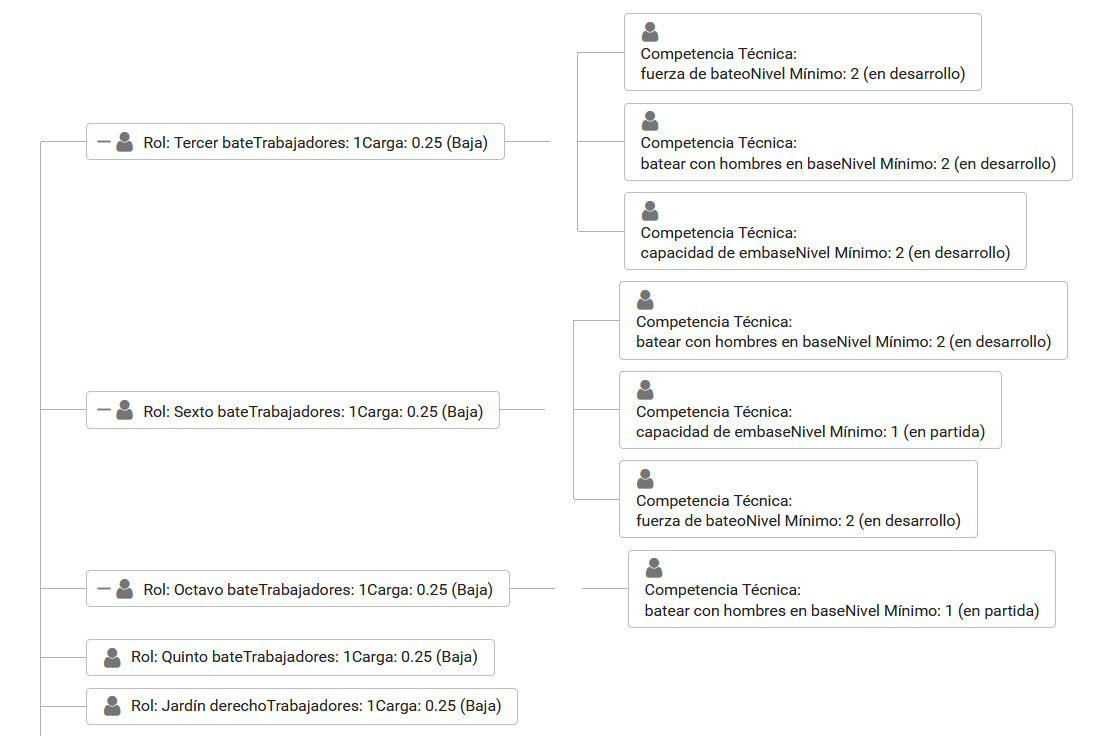
\includegraphics[width=\textwidth]{figuras/beisbol_conf_problema1.png}
	\caption{Trabajadores por rol y mínimo de competencias para desempeñar el rol} \label{fig:conf-equipo-pelota1}
\end{figure}

\begin{figure}[H]
	\centering
	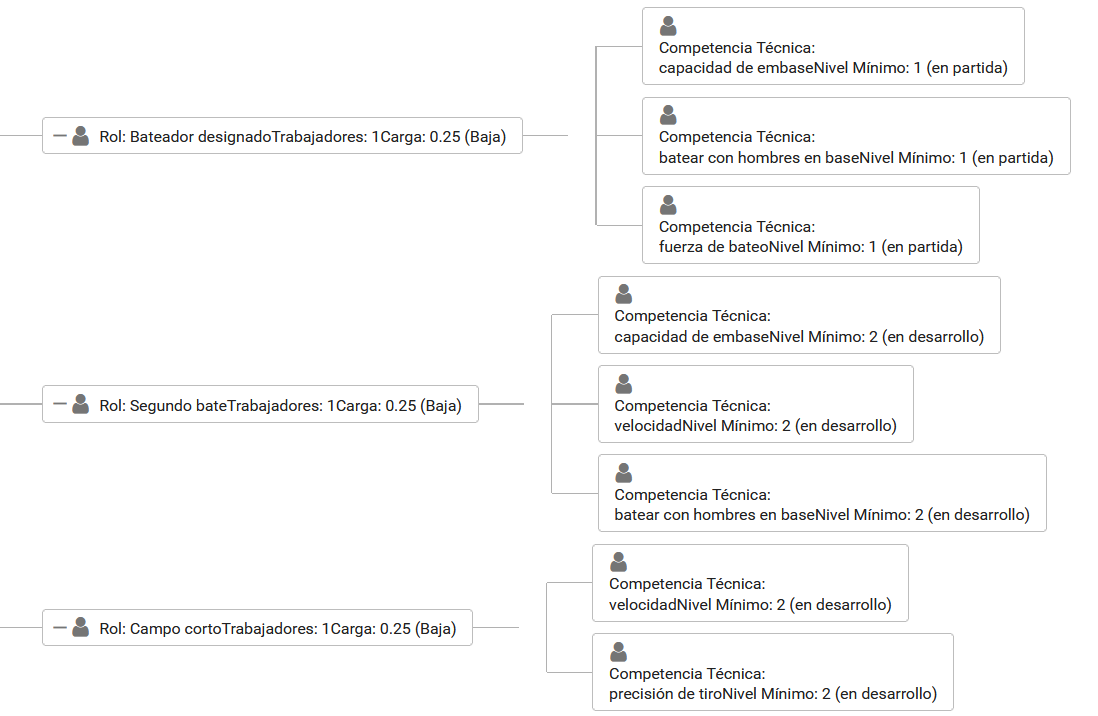
\includegraphics[width=\textwidth]{figuras/beisbol_conf_problema2.png}
	\caption{Trabajadores por rol y mínimo de competencias para desempeñar el rol} \label{fig:conf-equipo-pelota2}
\end{figure}

\begin{figure}[H]
	\centering
	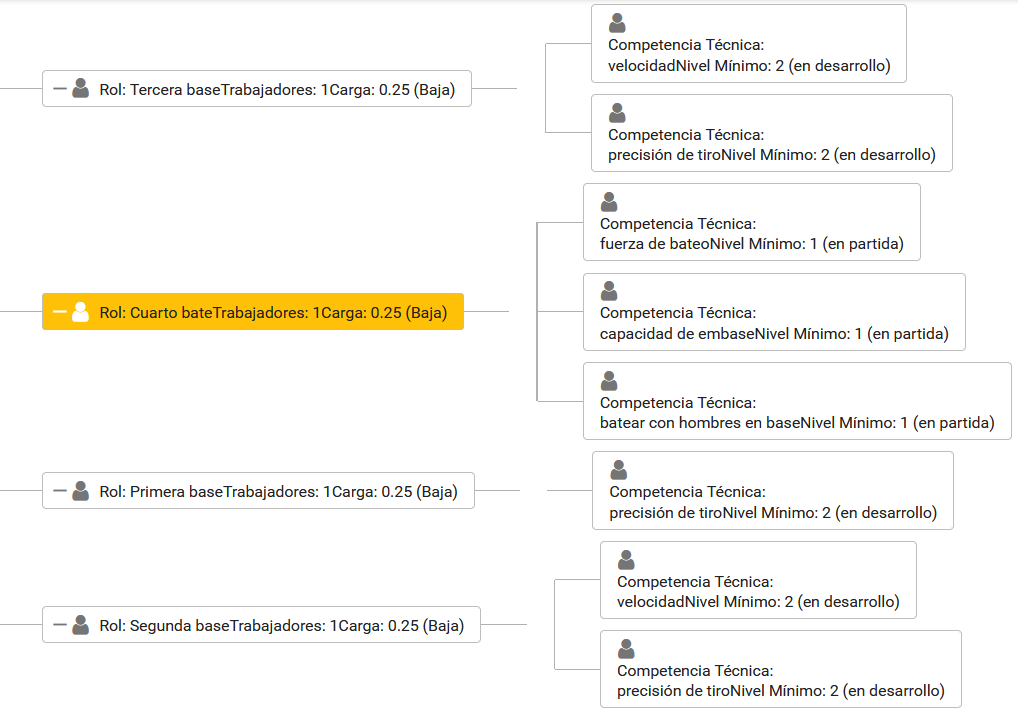
\includegraphics[width=.9\textwidth]{figuras/beisbol_conf_problema3.png}
	\caption{Trabajadores por rol y mínimo de competencias para desempeñar el rol} \label{fig:conf-equipo-pelota3}
\end{figure}

\begin{figure}[H]
	\centering
	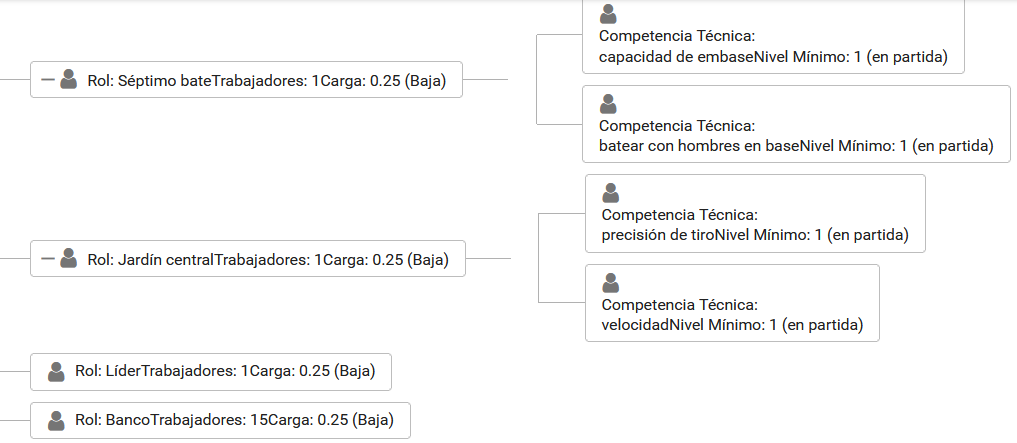
\includegraphics[width=.9\textwidth]{figuras/beisbol_conf_problema4.png}
	\caption{Trabajadores por rol y mínimo de competencias para desempeñar el rol} \label{fig:conf-equipo-pelota4}
\end{figure}

\chapter{Diagrama físico de la base de datos}
\begin{figure}[H]
	\centering
	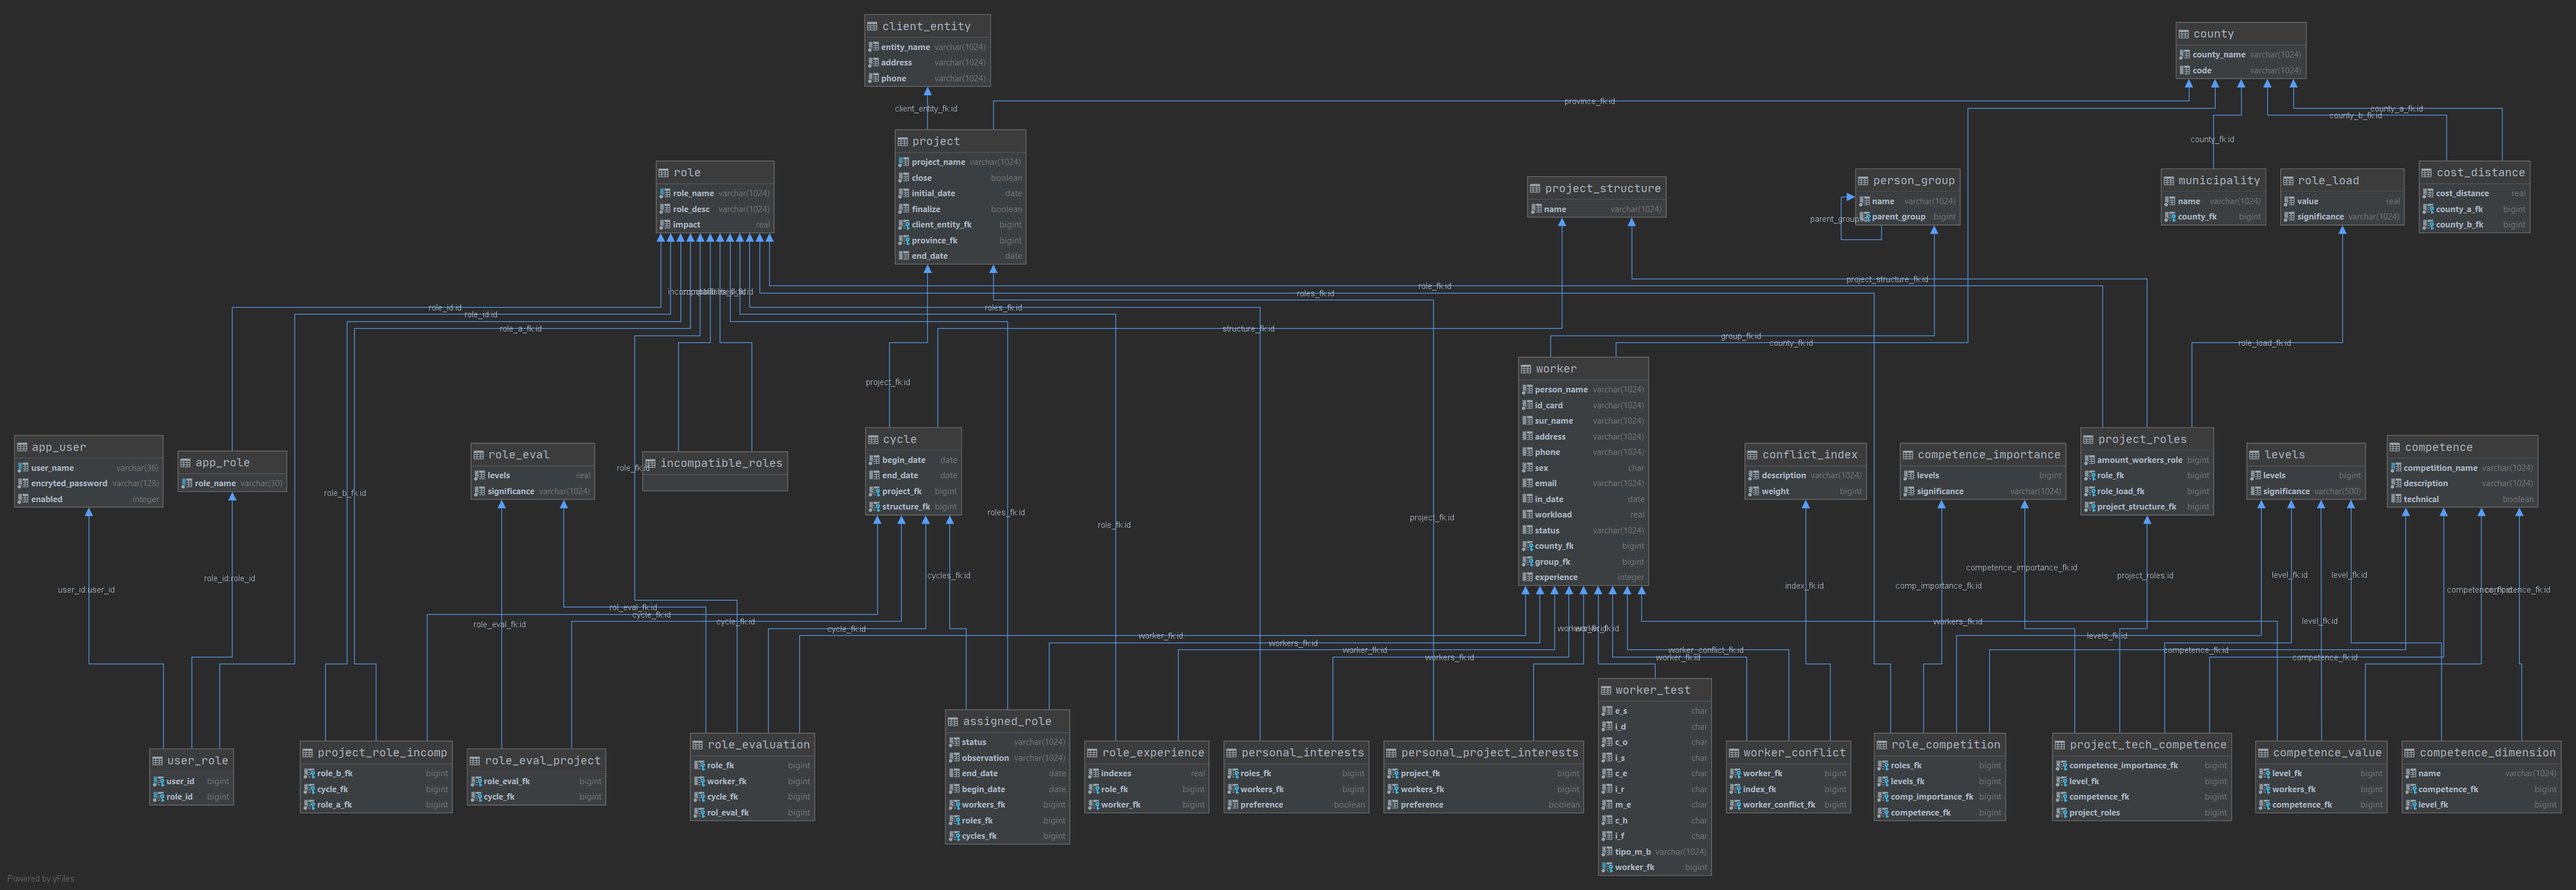
\includegraphics[width=\textwidth]{figuras/diagrama-base-datos.png}
	\caption{Diagrama físico de la base de datos de TEAMSOFT$^+$} \label{fig:diagrama-bd}
\end{figure}



\chapter{Algoritmos incorporados}


\begin{algorithm}[H]
	\caption{Restricción que verifica que una persona no pueda desempeñar menos roles que los definidos}
	%	\SetKwProg{Sol}{Restricci}{}{}
	\label{alg:rest-min-roles}
	%\Sol{($projects$)}{
	\KwIn {$state$ \tcp*[l]{estado que contiene los proyectos a verificar}
		\hspace{1.7cm}        $minRoles$ \tcp*[l]{Número obligatorio de roles a desempeñar} }
	\KwOut {$isRight$ \tcp*[l]{si todos los proyectos cumplen con la restricción}}
	%\LinesNumbered
	$projects = state$.getCode()\;
	$isRight = true$\;
	\ForEach{$project \in projects$}
	{$projectRoles = project$.getRols() \tcp*[l]{roles del proyecto}
		\ForEach{$rol \in projectRoles$}
		{
			$roleWorkers = rol$.getWorkers() \tcp*[l]{personas asociadas al rol}
			\ForEach{$worker \in roleWorkers$}
			{
				\If{$project$.getCantOccurenceWorker($worker$) $< minRoles$}{
					$isRight = false$ \tcp*[l]{no cumple con la restricción}
					\Break
				}
			}
			\If{$!isRight$} \Break
		}
		\If{$!isRight$} \Break
	}
	\Return $isRight$
	%}
\end{algorithm}

\clearpage

\begin{algorithm}[H]
	\caption{Restricción que verifica que el Líder del equipo ocupa otro rol como mínimo en el mismo equipo}
	\label{alg:restr-lider-rol}
	\KwIn {$state$ \tcp*[l]{estado que contiene los proyectos a verificar}}
	\KwOut {$isRight$ \tcp*[l]{si todos los proyectos cumplen con la restricción}}
	%\LinesNumbered
	$projects = state$.getCode()\;
	$isBossAssignedMoreThanOnce = false$\;
	\ForEach{$project \in projects$}
	{
		$isBossAssignedMoreThanOnce = false$\;
		$projectRoles = project$.getRols() \tcp*[l]{roles del proyecto}
		$roleBoss = project$.getProjectBoss()\;
		$projectRoles$.remove($roleBoss$)\;
		\ForEach{$rol \in projectRoles$}
		{
			$roleWorkers = rol$.getWorkers() \tcp*[l]{personas asociadas al rol}
			\ForEach{$worker \in roleWorkers$}
			{
				\If{$worker$.equals($roleBoss$.getWorkers().get(0))}{ \tcp*[l]{si el worker actual es igual al líder}
					$isBossAssignedMoreThanOnce = true$ \tcp*[l]{si cumple la restricción}
					\Break
				}
			}
			\If{$isBossAssignedMoreThanOnce$} \Break
		}
		\If{$!isBossAssignedMoreThanOnce$} \Break
	}
	\Return $isBossAssignedMoreThanOnce$
	%}
\end{algorithm}
\clearpage
\begin{algorithm}[H]
	\caption{Asignar personas de forma aleatoria a los roles, estableciendo que el líder juega más de un rol en los equipos}
	\label{alg:const-lider-rol}
	%\Sol{($projects$)}{
	\KwIn {$projects$ \tcp*[l]{Lista de proyectos sin asignación inicial}
		\hspace{1.7cm}        $limitPersonTries$ \tcp*[l]{Número de intentos de poner una persona en un rol} }
	\KwOut {$projects$ \tcp*[l]{Lista de proyectos con asignación inicial}}
	%\LinesNumbered
	\ForEach{$project \in projects$}
	{$rols = project$.getRols() \tcp*[l]{roles del proyecto}
		$boss = project$.getProjectBoss()\;
		$rols$.remove($boss$)\;
		\ForEach{$rol \in rols$}
		{$needs=rol$.getNeedWorked()\tcp*[l]{trabajadores necesarios en el rol}
			$count = 0$\;
			\While{$(needs > 0) \And (count < limitPersonTries)$}
			{
				$chosenPerson=$randomPersons()\tcp*[l]{seleccionar aleatoriamente una persona}
				\If{checkIndividualRestrictions($chosePerson,rol$)}
				{$rol=$.getWorkers().add(chosenPerson)\tcp*[l]{se añade si cumple las restricciones}
					$needs--$\;}
				\Else
				{
					$count++$\;}
			}
		}
		$rol$ = getRandomRol($rols$)\tcp*[l]{selecciona un Rol aleatoriamente}
		$worker$=getRandomWorker($rol$.getWorkers())\tcp*[l]{selecciona aleatoriamente un trabajador asignado a ese Rol}
		$boss$.getWorkers().add($worker$)\tcp*[l]{A ese trabajador se asigna el rol de Líder}
		$rols$.add($boss$)\;
	}
	%}
\end{algorithm}
\clearpage
\newgeometry{left=1.5cm,right=1.5cm,top=1cm,bottom=1cm} 
\scalebox{.92}{
\begin{algorithm}[H]
	\caption{Asignar personas aleatoriamente a roles con la restricción de 2 roles mínimos.}
	%  \SetKwProg{Sol}{SolucionInicial2}{}{}
	\label{alg:2}
	%  %\Sol{($projects$)}{
	\KwIn {$projects$ \tcp*[l]{Lista de proyectos sin asignación inicial}
		\hspace{1.7cm}$limitPersonTries$ \tcp*[l]{Intentos de poner una persona en un rol} 
		%\hspace{1.7cm} $minRolePerson$  \tcp*[l]{Número mínimo de roles que desempeña una persona en un proyecto}
	}
	\KwOut {$projects$ \tcp*[l]{Lista de proyectos con asignación inicial}}
	%\LinesNumbered
	$allWorkers=$getWorkerAvailable()\tcp*[l]{Obtener trabajadores disponibles} 
	\ForEach{$project \in projects$}
	{$rols = project$.GetRols() \tcp*[l]{roles del proyecto}
		$assignedWorkers = {}$\tcp*[l]{ workers asignados con el número mínimo de roles}
		$assignedRoleWorkers= {}$\tcp*[l]{ roles con todos los trabajadores asignados}
		$existWorkers = true$ \tcp*[l]{existen trabajadores disponibles}
		$existCompatibleRole = true$ \tcp*[l]{existen roles compatibles disponibles}
		\tcc{mientras existan disponibilides}		
		\While{$\mbox{\rm existAvailableRoles}(allProjectRoles,assignedRoleWorkers) \And existWorkers$} {
			\tcc{selecciona aleatoriamente un trabajador disponible}
			$workerToAssign =$ getRandomNotAssignedWorker($allWorkers$, $assignedWorkers$)\;
			\If{ $workerToAssign \neq null$} 
			{\tcc{existe un trabajador disponible}
				$roleToAssign = $getRandomAvailableRole($allProjectRoles$, $assignedRoleWorkers$\tcp*[l]{rol con trabajadores por asignar}
				$compatibleRole =$ getRandomCompatibleRole($rols$, $roleToAssign$, $assignedRoleWorkers$)\tcp*[l]{roles compatibles con $roleToAssign$ no asignados}
				\If{$compatibleRole \neq null$} { 
					\tcc{si hay rol compatible asigna el worker a los roles}
					$roleToAssign.$getWorkers().add($workerToAssign$)\;
					$compatibleRole.$getWorkers().add($workerToAssign$)\;
					$assignedWorkers.$add($workerToAssign$)\tcp*[l]{worker asignado}
					\tcc*{los roles satisfacen su demanda de trabajadores})
					\If {$roleToAssign.$getWorkers().size() =$roleToAssign.$getNeededWorkers()}{ 
						$assignedRoleWorkers.$add(roleToAssign)\;}
					\If{$compatibleRole.$getWorkers().size() == $compatibleRole.$getNeededWorkers()} {
						$assignedRoleWorkers.$add($compatibleRole$)\;
					}
				} 
				\Else{$existCompatibleRole = false$\;
				}
			} 
			\Else{$existWorkers = false$\;}
		}
		
		\If{$existWorkers \And existCompatibleRole$} {
			$projectBoss=rol$.getProjectBoss()\;
			
			$boss=$getRandomPerson($assignedWorkers$)\;
			$projectBoss$.getWorkers().add($boss$);
		}
	}
\end{algorithm}
}
\restoregeometry 
\begin{algorithm}[H]
	\caption{Operador de sustitución}
	\label{alg:operador-sustitucion}
	\KwIn {$projects$ \tcp*[l]{listado de equipos} \hspace{1.7cm} $codificacion$ \tcp*[l]{configuración del problema}
	}
	\KwOut {lista de proyectos actualizada}
	$randomProject = getRandomProject(projects)$  \tcp*[l]{obtener equipo aleatorio}
	$allProjectRoles = randomProject$.getRoleWorkers()  \tcp*[l]{escoger un rol aleatorio}
	$allWorkers = codification$.getSearchArea()  \tcp*[l]{workers disponibles}
	
	\If{$!allProjectRoles.isEmpty()$}{ 
		$randomRole = getRandomRole(allProjectRoles)$ \;
		$randomWorkerOfSelectedRole = getRandomWorkerByRole(randomRole)$\;
		$workerToSwap=getRandomWorker(allWorkers)$ \;
		\ForEach{$roleWorker \in allProjectRoles$}
		{
			\ForEach{$worker \in roleWorker.getWorkers()$}
			{
				\If{$worker$.equals($randomWorkerOfSelectedRole$)}{
					$roleWorker$.getWorkers().replace(worker, randomWorkerOfSelectedRole)			\;			
				}			
			}	
		}
	}
\end{algorithm}
}

